\chapter{Experimentación}

\section{Beacons y configuración}

Los beacons utilizados corresponden a beacons de la marca Kontakt, y el numero es 8, sin embargo, no son todos iguales. Esto ayuda a comprobar que tan efectivo es utilizar distintos modelos, ya que en entornos reales, por ejemplo en una mina, es sumamente importante contar con beacons bluetooth que se adapten al espacio físico en donde son dispuestos, por ejemplo si es necesario instalarlos en una oficina, los beacons convencionales funcionan de buena manera, sin embargo en ambientes hostiles como lugares con polvo o de difícil acceso, es necesario contar con beacons preparados para estas dificultades, los cuales tengan baterías de larga duración, sean anti polvo y agua, entre otras características. A continuación se muestra el resumen de los beacons utilizados:

\begin{enumerate}
\item \textbf{Beacon: } Beacon mas popular y de menores prestaciones. Es el clásico Beacon vendido por la compañía Kontakt. Posee una batería con duración de hasta 48 meses y un rango de 70m. Se utilizan 4 unidades.

\item \textbf{Beacon Pro: } Beacon con mas funciones de seguridad, ahorro de bateria, sensores de luz y a prueba de agua. Hasta 60 meses de bateria y rango de 70m. Se utilizan 2 unidades.

\item \textbf{Tough Beacon: } Hasta 24 meses de batería y rango de 70m. A prueba de polvo y agua. Especialmente diseñado para condiciones extremas.


\end{enumerate}

Cabe destacar que las caracteristicas basicas del \textit{Hardware} de cada beacon son las presentes en la comparativa realizada en la sección \ref{sec:seleccion}.

Foto beacons.

Lo siguiente es definir la configuración de cada Beacon. Los parámetros mas relevantes en este caso serian el \textit{TX Power} y el \textit{Beacon Interval}. En un despliegue real, lo mas relevante es disminuir los costos, que en este caso están asociado a las baterias o mas bien al cambio de estas a lo largo del tiempo. Estos dos parametros son importantes para la localización indoor, ya que el TX Power define la potencia de salida de cada Beacon y el intervalo corresponde a cada cuanto un beacon envía un mensaje a los dispositivos bluetooth cercanos. 

El valor de Tx Power afecta principalmente a tres factores claves, estos son el rango de la señal, es decir, la distancia maxima alcanzada; el segundo corresponde a la estabilidad de la señal y finalmente la bateria, aunque este ultimo factor es mayormente influenciado por el intervalo.

En terminos simples, TX Power representa que tan poderosa es la señal transmitida por los beacons en dBm y corresponde a un numero dentro del rango 0-7, donde 0 es menos poderoso y 7 el mas poderoso.Es claro que mientras mas poderoso es la señal, mayor rango alcanza y mas estable es la señal, sin embargo el consumo de energia aumenta significativamente. Para determinar el parametro TX power entonces es necesario tener en cuenta estos factores. Para el caso del posicionamiento indoor, es claro que el rango debe ser maximo, ya que de esta forma la señal de cada Beacon puede alcanzar a la gran parte de los usuarios de la zona. El otro punto significativo es establecer que tan seguido es necesario cambiar las baterias. Este punto es relevante para despliegues a gran escala y depende en gran medida de las organizaciones interesadas en desplegar un sistema de este tipo. Finalmente, es importante considerar la interferencia subyacente debido al entorno, por ejemplo objetos contundentes o multiples personas, en este caso se requiere una señal mas potente para cortar de esta forma la interferencia y pasar a traves de esta. Por los motivos declarados anteriormente se decide utilizar un TX Power igual a 7, o equivalentemente 4 dBm.

Con respecto al intervalo utilizado, es un parámetro de mucho mayor relevancia que el TX Power para el tipo de problema a resolver. Esto se debe principalmente a que el intervalo corresponde a que tan frecuente es transmitido un paquete desde un Beacon a un dispositivo móvil. Considerando que el posicionamiento debe ser lo mas cercano a  tiempo real, la información debe ser suministrada lo mas rápidamente posible. El intervalo es medido en milisegundos, y como es esperable, mientras mas pequeño el intervalo, mas recurrente es la comunicación pero mayor es el consumo de batería. A pesar de que el intervalo sea muy pequeño, muchas veces los sistemas operativos no son capaces de recibir tan rápidamente estas señales, debido a limitaciones de seguridad u otras configuraciones del fabricante como es el caso de Apple. En Android estas limitaciones no existen y por lo tanto puede recibir todas las señales, pero esto afecta de forma significativa la batería del teléfono. Por otra parte, mientras menor es el intervalo, mayor es la estabilidad de la señal, ademas el intervalo afecta significativamente a el posicionamiento en interiores, debido a que mientras mas rápido se mueve un usuario, si el intervalo es demasiado alto, su posición sufrirá saltos o cortes que no muestran realmente la ruta de desplazamiento. Si el intervalo es pequeño, puede detectar mas fácilmente la posición del usuario en cada momento con precisión de unos pocos centímetros. La  ejemplifica esta situación:


\begin{figure}[ht!]
\centering
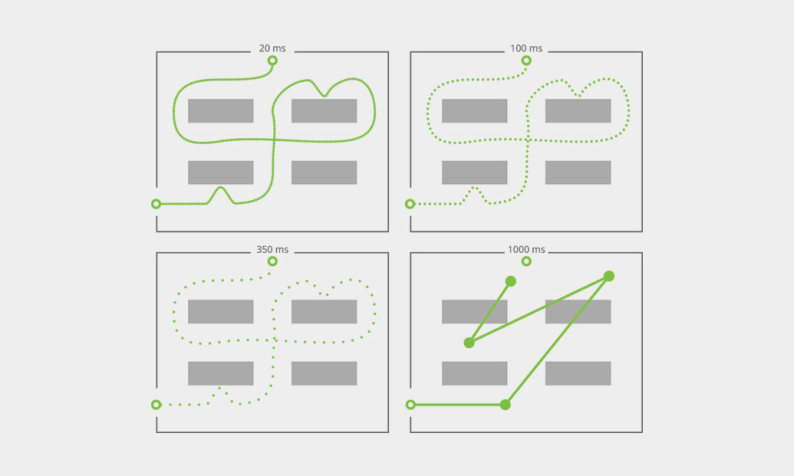
\includegraphics[width=.6\textwidth]{figures/interval.jpg}
\caption[abs]{Posicionamiento indoor con diferentes intervalos de aviso en mili segundos\\
{\scriptsize (Fuente: \cite{interval})}}
\label{fig:intervalo}
\end{figure}

Por lo anterior, es claro que los parámetros seleccionados deben ser el mayor valor posible para el TX Power correspondiente a 7, y un valor del intervalo igual a 100ms. Para configurar estos parámetros, Kontakt dispone de una aplicación para dispositivos Android. La \autoref{fig:kontaktapp1} y \ref{fig:kontaktapp2} muestran como han sido configurados los Beacons. Esta configuración es idéntica para todos los beacons utilizados.


\begin{figure}[ht!]
\centering
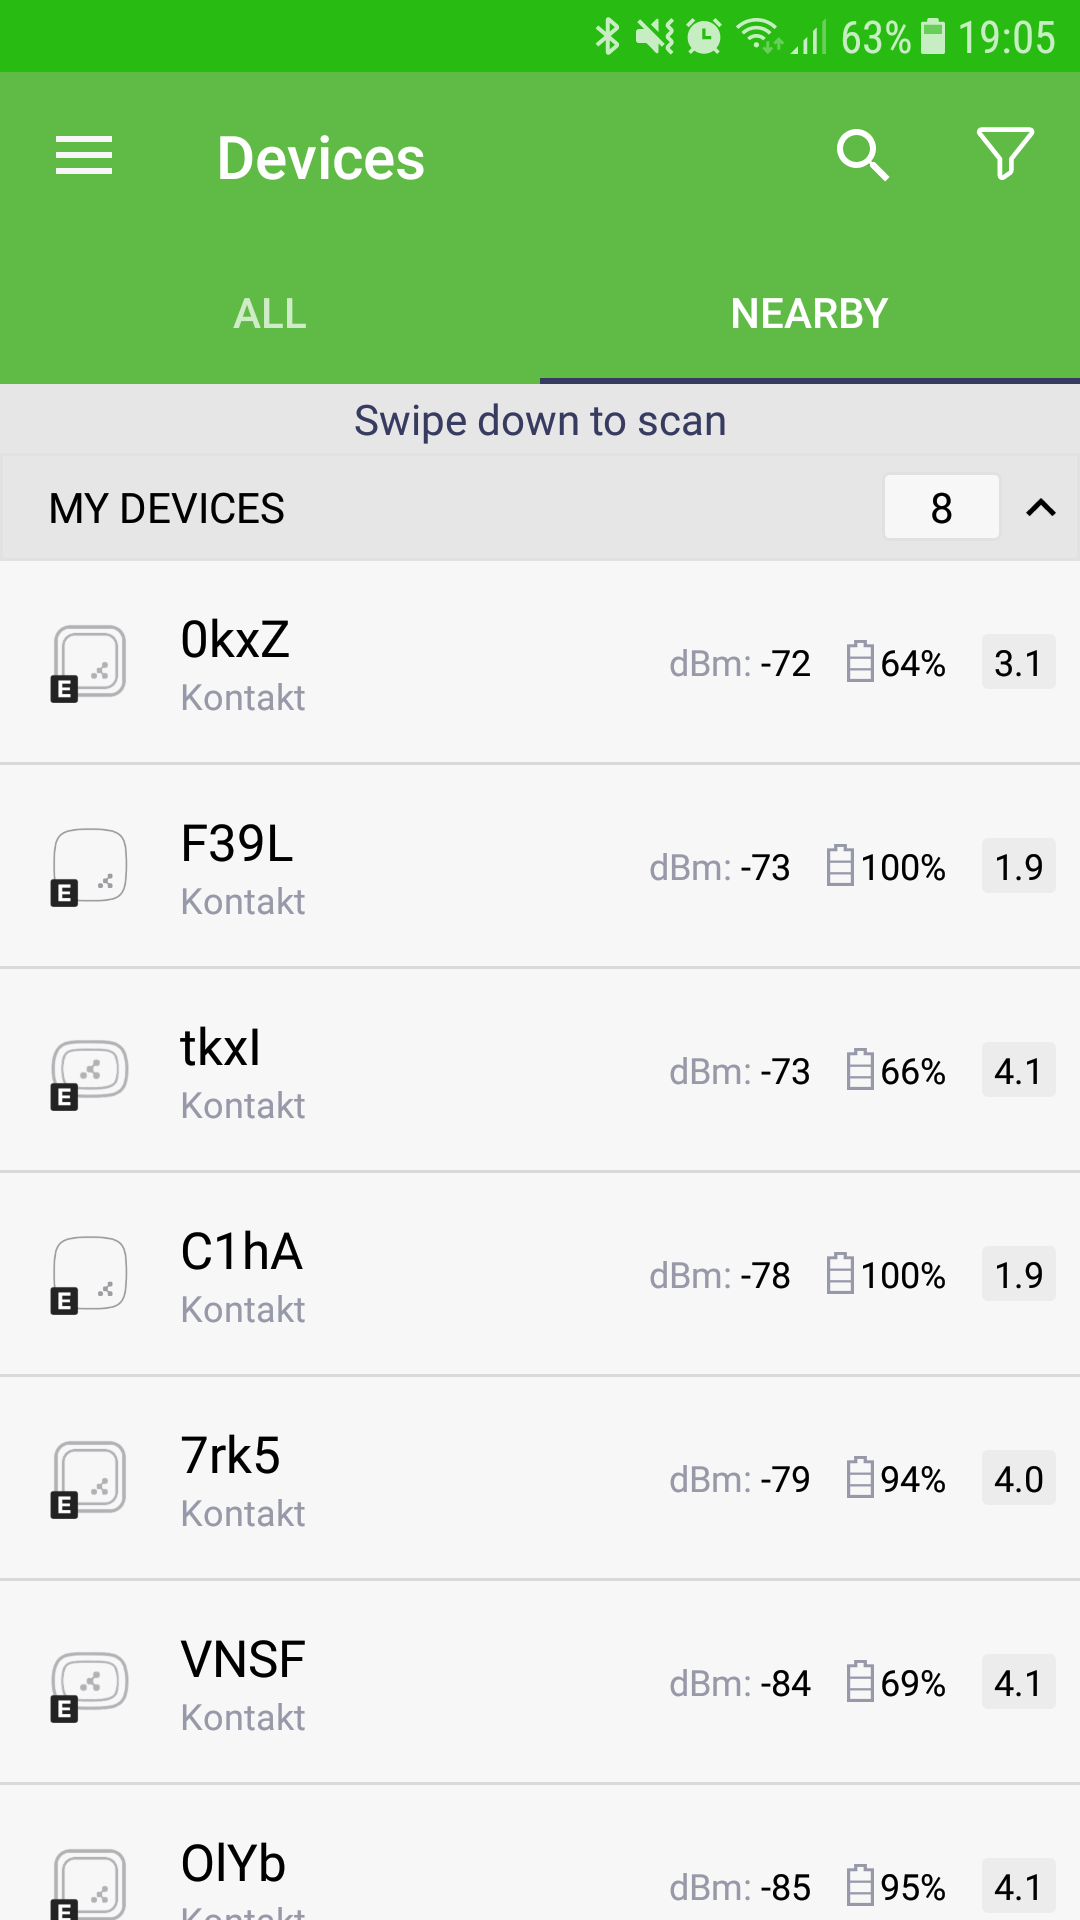
\includegraphics[width=.3\textwidth]{figures/kontaktapp1.png}
\caption[abs]{Listado de los beacons encontrados para su posterior configuración\\
{\scriptsize (Fuente: Elaboración Propia)}}
\label{fig:kontaktapp1}
\end{figure}

\begin{figure}[ht!]
\centering
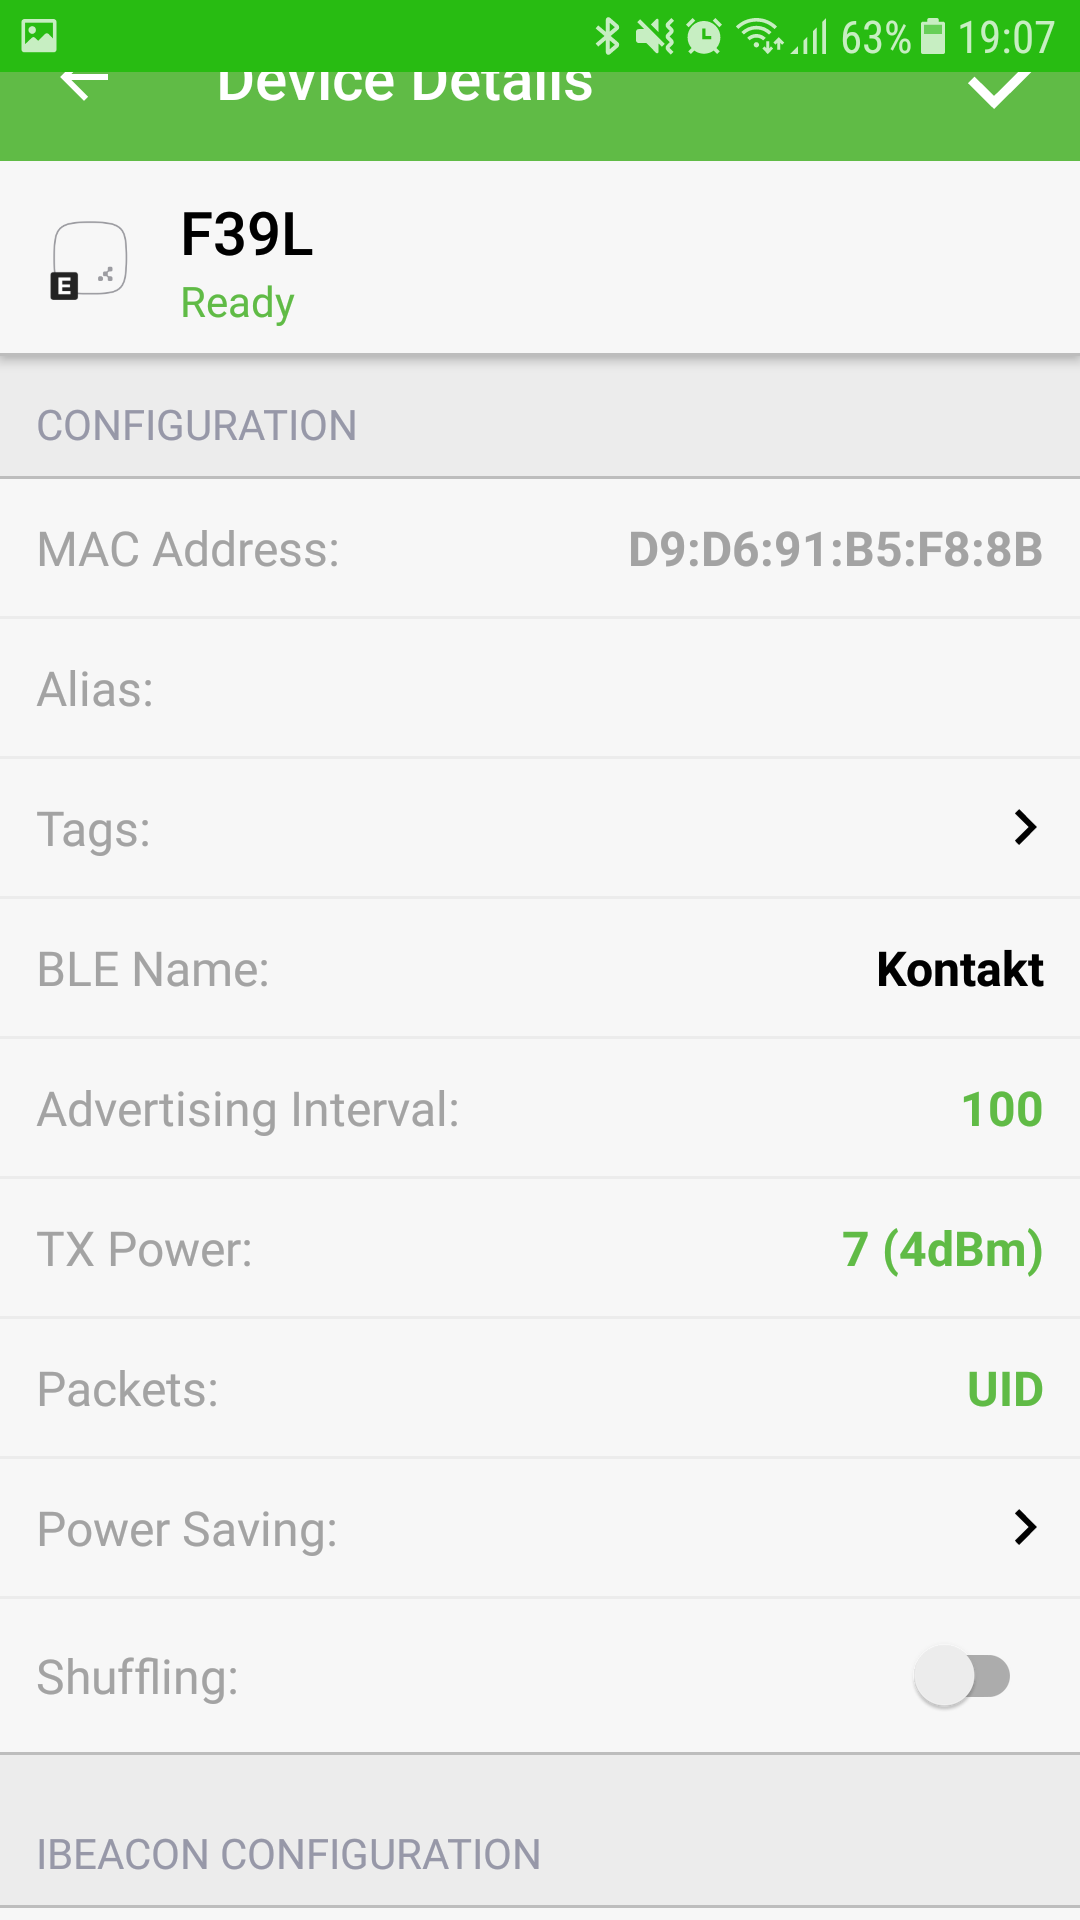
\includegraphics[width=.3\textwidth]{figures/kontaktapp2.png}
\caption[abs]{Configuración que ejemplifica los valores definidos para TX Power y el intervalo de transmisión\\
{\scriptsize (Fuente: Elaboración Propia)}}
\label{fig:kontaktapp2}
\end{figure}

Ademas, los protocolos utilizados son UID de Eddystone por su flexibilidad y transversalidad para los múltiples dispositivos móviles existentes en el mercado.

\section{Lugar de experimentacion}

Para realizar los experimentos, se decide utilizar un lugar en donde las condiciones sean adversas y cambiantes, debido al alto transito de objetos y ademas no se presenten señales GPS. Por lo anterior, se decide utilizar el estacionamiento subterráneo de la universidad Técnica Federico Santa Maria, Campus San Joaquin, ubicado en Vicuña Mackenna 3939. Las dimensiones constan de $144.75m$ de largo y $36m$ de ancho. La \autoref{fig:estSubterraneo} muestra el plano del estacionamiento a escala.

\begin{figure}[ht!]
\centering
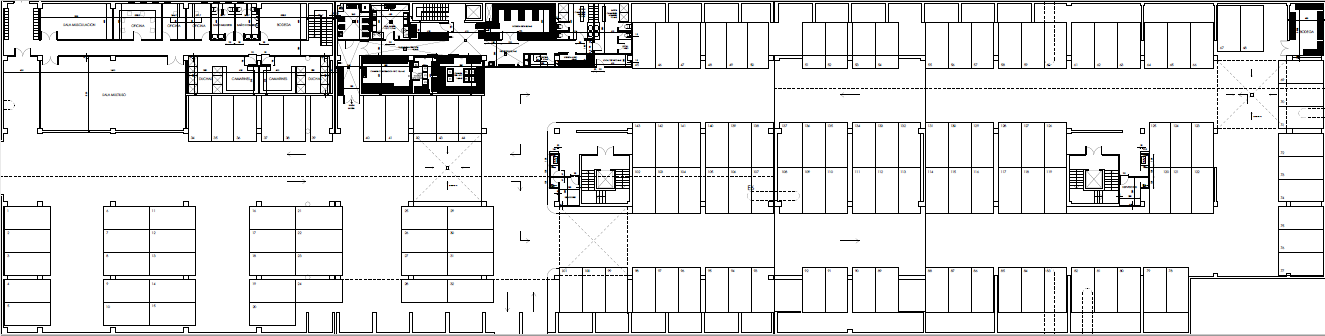
\includegraphics[width=.6\textwidth]{figures/estSubterraneo.png}
\caption[abs]{Plano del estacionamiento subterraneo de la Universidad Federico Santa Maria\\
{\scriptsize (Fuente: Elaboración Propia)}}
\label{fig:estSubterraneo}
\end{figure}

Este lugar es ideal para realizar pruebas, ya que presenta interferencia debido a los vehiculos en transito y la disposicion de los objetos es cambiante. Ademas, se pueden obtener mediciones con ruido producto de la reflexion de las ondas, lo que pone a prueba a los algoritmos de clasificación para detectar estos patrones. 

\begin{figure}[ht!]
\centering
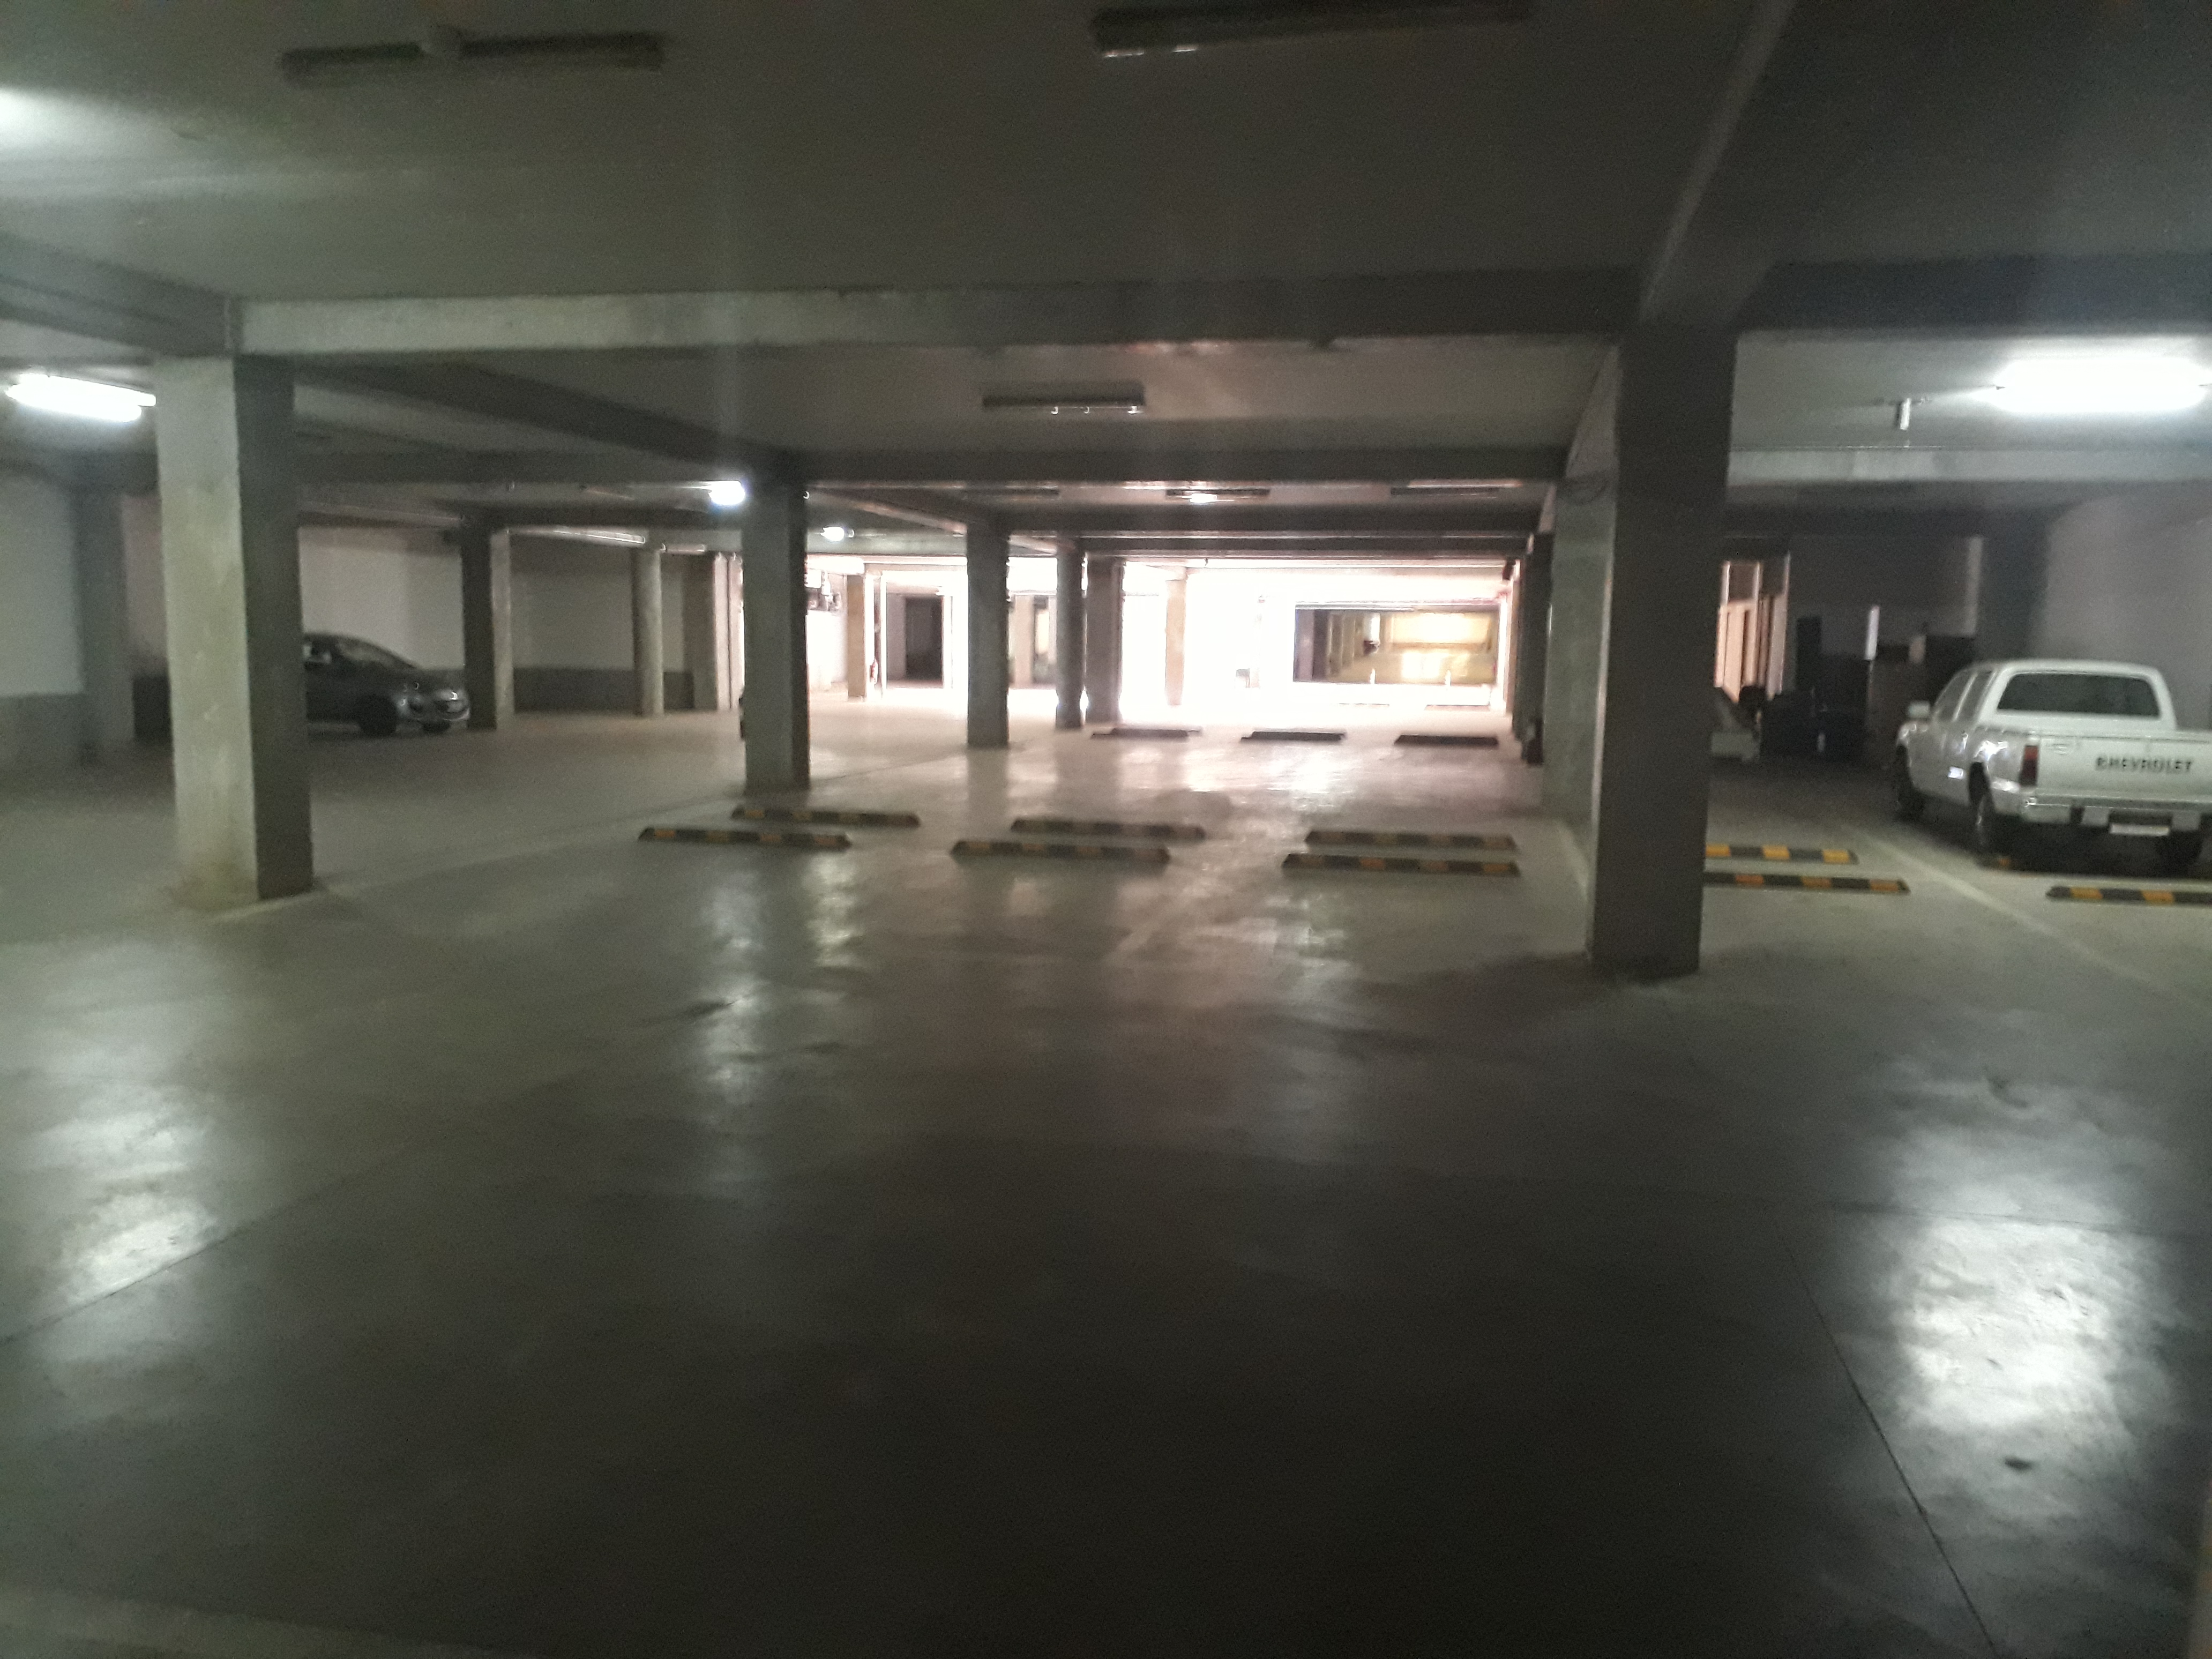
\includegraphics[width=.6\textwidth]{figures/estReal.jpg}
\caption[abs]{Fotografía del espacio de experimentación real, correspondiente al estacionamiento subterraneo\\
{\scriptsize (Fuente: Elaboración Propia)}}
\label{fig:estReal}
\end{figure}


\section{Software Utilizado}

\subsection{Descripción de la aplicación}

La aplicación desarrollada es construida para el sistema operativo Android. Para su desarrollo se utiliza Android Studio \footnote{\url{https://developer.android.com/studio/index.html}}, es IDE oficial para el desarrollo de aplicaciones nativas. El numero de compilación corresponde a $3.0.1$. La selección de este sistema operativo es debido a su fácil acceso y prácticamente ningún costo debido a licencias, ya que es basado en linux por lo que su desarrollo es gratuito, al igual que la distribución de aplicaciones, por lo que es mucho mas efectivo para el desarrollo de una aplicación de prueba bajo un entorno controlado.

Los requisitos básicos de la aplicación construida son los siguientes:

\begin{itemize}
\item Mostrar el plano del lugar de experimentación, el cual funciona como base para posicionar los demás elementos.

\item Permitir la adición de nuevos dispositivos Beacons con su respectivo marcador. Para ello debe detectar automáticamente el beacon mas cercano y sugerir este para su inserción en el mapa.

\item Permitir la captura de datos, es decir, los nuevos fingerprints, en donde el usuario es quien provee la posición exacta y la aplicación mide los valores RSSI durante un periodo de tiempo, para posteriormente almacenarlos en la base de datos. 

\item Modificar los valores de intervalo y el numero de mediciones en cada punto, el cual puede también definirse en periodo de tiempo.

\item Tener una base de datos \textit{SQLite}, la cual permite la persistencia de los datos. También se debe poder transformar esta base de datos a un archivo CSV.

\item Para la etapa online, debe permitir seleccionar el algoritmo a utilizar y mostrar en tiempo real la posición del usuario según el algoritmo usado. Por otra parte, debe guardar estos resultados en un archivo de texto para su posterior análisis.



\end{itemize}

La aplicación construida consta de 3 secciones principales las cuales ayudan a todas las etapas del modelo fingerprint, estas son \textbf{Offline}, \textbf{Online} y \textbf{Configuración}. Estas son descritas a medida que se desarrolla el proceso de la experimentación.


\subsection{scikit-learn}

Para la elaboración de modelos de clasificación, una de las librerías mas utilizadas es scikit-learn o tambien conocida como SKlearn \cite{scikit-learn}, la cual es una completa API para elaborar y realizar maquetas de machine learning. Su core esta basado en python y para su uso se utiliza el siguiente entorno de desarrollo:

\begin{itemize}
\item Anaconda 1.6.2
\item Jupyter Notebook 5.0.0
\item scikit-learn 0.18.2
\item Python 3.6.1
\end{itemize}

Las principales ventajas de utilizar SKlearn son obtener modelos simples y eficientes, que estan muy avanzados y que presentan una comunidad dedicada a su correcto funcionamiento. Ademas esta construida sobre 3 de las librerías mas utilizadas en Python en el contexto de desarrollo científico, como son NumPy, SciPy y Matplotlib. Por otra parte su licencia es de codigo abierto, por lo que cualquiera puede utilizar y modificar el código sin restricciones.

A pesar que en este caso solo se utilizara para los algoritmos de clasificación, PCA y gráficos, también presenta herramientas que agilizan el desarrollo como por ejemplo lectura de archivos, funciones de normalizacion establecidas, funciones de puntuación o accuracy, pre procesamiento de datos, entre otras. También sirve como herramienta de regresión, minería de datos y análisis de datos.

\section{ Tensorflow}

A pesar que SKlearn presenta tantas ventajas para el desarrollo agil de modelos de maquinas de aprendizaje, no es tan bueno en redes neuronales, y no implementa la mayor parte de los algoritmos modernos en este campo. Esto se debe principalmente a que todo el core de SKlearn es python, y se vuelve sumamente lento para entrenar este tipo de redes, sobre todo redes profundas. Para resolver este problema, se decide utilizar Tensorflow \cite{tensorflow2015-whitepaper}, un completo framework de desarrollo de Google, que con respecto a SKlearn es mucho menos intuitivo y de fácil uso al usuario final, ya que su programacion es de mucho mas bajo nivel y requiere conocimiento avanzado de los algoritmos que se quieren implementar.  Mucha veces se describe como las piezas fundamentales para la creacion de algoritmos de maquinas de aprendizaje, como si fueran Legos, no asi SKlearn, el cual ya esta todo listo, solo debe ser utilizados y configurar los parametros de los algoritmos.

Tensorflow es una biblioteca de código abierto y su principal ventaja es que a pesar que la parte superior esta basada en python, esta se comunica internamente a código compilado en C++, lo cual lo vuelve sumamente eficiente. Ademas, por la forma en que Tensorflow representa los datos, es decir, tensores o arreglos multidimensionales, y las operaciones referentes a grafos sin estado que transforman estos tensores, lo vuelve increíblemente rapido para entrenar y desplegar, incluso presenta API para dispositivos moviles en Java, C++ y GO, en donde solo se porta el grafo construido y se puede realizar inferencia en equipos de muy pocos recursos, lo que lo vuelve una alternativa ideal para desarrollar redes neuronales profundas, utilizando  pocos recursos en el sistema operativo Android. A pesar de que presenta operaciones de bajo nivel, igualmente tiene disponible la opcion de API de alto nivel, como por ejemplo implementar redes convolucionales o redes profundas en un par de lineas de codigo Python, conocidos como estimadores de alto nivel.

Finalmente tensorflow basa todo su procesamiento en el grafo computacional mencionado anteriormente, el cual consiste en una serie de operaciones de tensores dispuestos en un grafo de nodos. Luego de que se arma este grafo de operaciones, se puede entrenar mediante las operaciones incluidas en tensorflow, llamados optimizadores, como lo son gradiente descendente. El paso final es utilizar este grafo computacional para probar los modelos y utilizarlos en despliegues reales.


\section{Recolección de fingerprints}


Con todo lo anterior en cuenta, es necesario definir que tipo de dispositivo móvil y sistema operativo se utilizara para colectar los datos en cuestión, que finalmente se transformaran en fingerprint dando lugar al radiomap. En este caso, el dispositivo a utilizar es un dispositivo Samsung Galaxy J7 Prime, que dentro de sus prestaciones posee una CPU Octa-core 1.6 GHz Cortex-A53, una GPU Mali-T830 MP1, 3GB de memoria ram interna y el tipo de Bluetooth corresponde a 4.1 LE. Con respecto a su sitema operativo, es Android 7.0 Nougat el cual no presenta limitaciones en la lectura de las señales Bluetooth por lo que puede recepcionar las señales tan rápido como estas son emitidas.

Definido esto, lo siguiente establecer la forma en que deben ser posicionados los beacons y ademas como funciona la recolección de fingerprints como tal. Para el posicionamiento de los Beacons, se decide utilizar una estrategia de grilla, esto es, ubicarlos de manera equidistante en las esquinas del plano. Ademas, para este trabajo se debe considerar que el plano completo no fue inspeccionado debido a que la densidad de los beacons seria muy baja para lograr óptimos resultados, por lo que finalmente se decide utilizar los 8 beacons en un área reducida del estacionamiento y ubicar cada beacon a una distancia de 16 metros a sus vecinos adyacentes formando esta especie de grilla. Finalmente, el área efectiva a utilizar se calcula según las dimensiones de 16 metros de ancho por 44 metros de largo, con lo que se obtiene un área de $704m^2$. Cabe destacar que un par de beacons fueron ubicados respecto a sus vecinos a una distancia de 12 metros y no 16, debido a la disposición del estacionamiento.  Lo anterior define un cuadrilátero de esquinas $ \{(0,6), (0, 22), (44,22) , (44,6)\} $, Notar que el valor de $Y$ comienza en $6$ y no en $0$, debido a dificultades en el lugar de experimentación.

Con respecto al punto de recolección de fingerprints, se desarrolla una aplicación para el sistema operativo Android, y se decide utilizar una grilla para los puntos de medición o referencia de 4 metros por 4 metros, es decir, cada punto de medición esta en medio de cada celda de esta grilla, consiguiendo de esta manera un total de 44 puntos de referencia. La \autoref{fig:deployBeacons} muestra esta situación.


\begin{figure}[ht!]
\centering
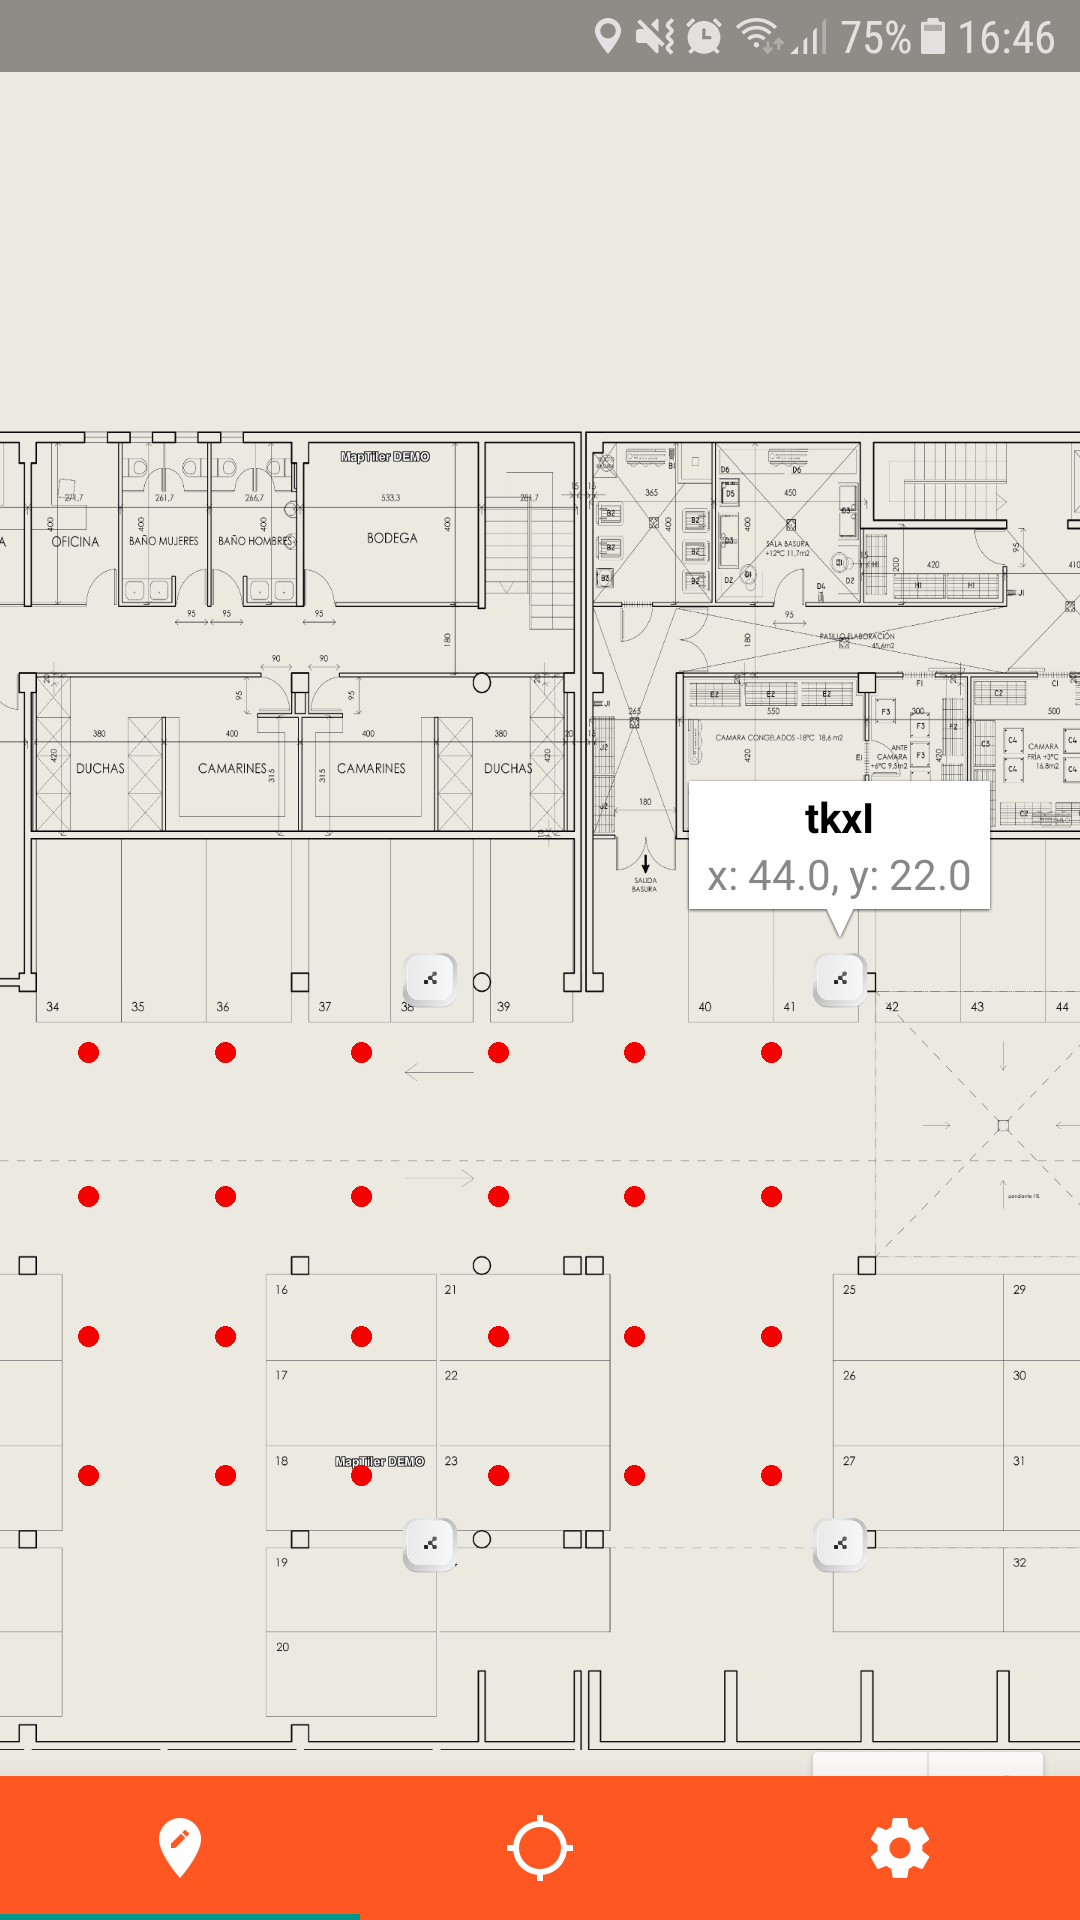
\includegraphics[width=.3\textwidth]{figures/deployBeacons.png}
\caption[abs]{Disposicion de beacons y puntos de referencia dentro de la grilla, utilizando la aplicacion Android\\
{\scriptsize (Fuente: Elaboración Propia)}}
\label{fig:deployBeacons}
\end{figure}

La aplicación consta de una sección offline, en donde se pueden incorporar nuevos Beacons a la base de datos \textit{sqlite}(base de datos por defecto en dispositivos Android), ademas de poner realizar  la captura de datos o fingerprints, definiendo la ubicación actual según algún patrón o posición exacta. Otro punto importante a considerar es el numero de fingerprints a obtener en cada punto de referencia. Considerando el intervalo de emisión de cada Beacon, es necesario establecer un tiempo alto para notar cambios en el lugar de experimentación, por lo que se define una ventana de tiempo de 5 minutos en cada punto de referencia. Sin embargo, para obtener mejores resultados y en vista y considerando que las maquinas de aprendizaje aprenden de mucho mejor manera con datos variados, se decide inspeccionar y recolectar datos a través de diferentes días, con el objetivo de que sea mas fácil para los algoritmos encontrar patrones eventualmente. Finalmente se seleccionan 150 mediciones por punto de la grilla, seleccionando una medición cada dos segundos para tener menor información repetida y no sobremuestrear la base de datos.

Una vez recolectados los datos, se obtiene una base de datos \textit{SQLite} con figerprints, la cual presenta 6600 registros, en donde los dos primeros campos representan la posicion de X y la posicion de Y respectivamente, y los siguientes 8 campos corresponden a los Beacons detectados con su respectiva intensidad de la señal o RSSI. Por lo anterior, las clases definidas para X son $ X \in [2, 6, 10, 14, 18, 22, 26, 30 , 34, 38, 42]$ y para $Y \in [8, 12, 16, 20]$ con  un total de 11 clases para $X$ y 4 clases para $Y$ . Recordando que estas clases representan el centro de la grilla con celdas cuadradas de 4 metros, es decir el punto medio de estas, por lo que para $ X$, la primera clase se define según el punto inicial,  el cual es cero, ademas el  punto medio de la primera celda es la mitad de la dimension total, es decir, 2 metros que representa la primera clase y asi se construyen las siguientes clases, adicionando 4 metros(cambio de celda). Para $Y$ se debe tener en consideración que la primera clase es 8, esto se debe principalmente a que los valores de $ Y$ no comienzan precisamente en cero, debido a dificultades en la posición de objetos dentro del estacionamiento, por lo que se decide iniciar en $Y = 6$, con lo que el primer punto es este valor inicial mas la mitad de la grilla(2), es decir 8.  Un punto importante a definir es que valor asignar a los beacons que no han sido detectados, en este caso y como el valor RSSI no puede ser mayor a cero, se decide asignar un valor de 100 dBm como un identificador de que no se ha detectado señal.

Con esta base de datos es posible construir otros tipos de archivos, que resuman todos los fingerprints detectados. Esto se realiza ya que para los algoritmos de machine learning existen muchas mas librerías dedicadas a leer datos en formatos mas convencionales como TXT o CSV. Por lo mismo, en la aplicación se define una sección de configuración para transformar y almacenar esta base de datos en formato CSV o \textit{comma-separated values}.  La \autoref{fig:configApp} muestra esta pestaña de configuracion, incluyendo el numero de mediciones y las opciones de exportar la base de datos, transformarla a CSV o eliminarla.

\begin{figure}[ht!]
\centering
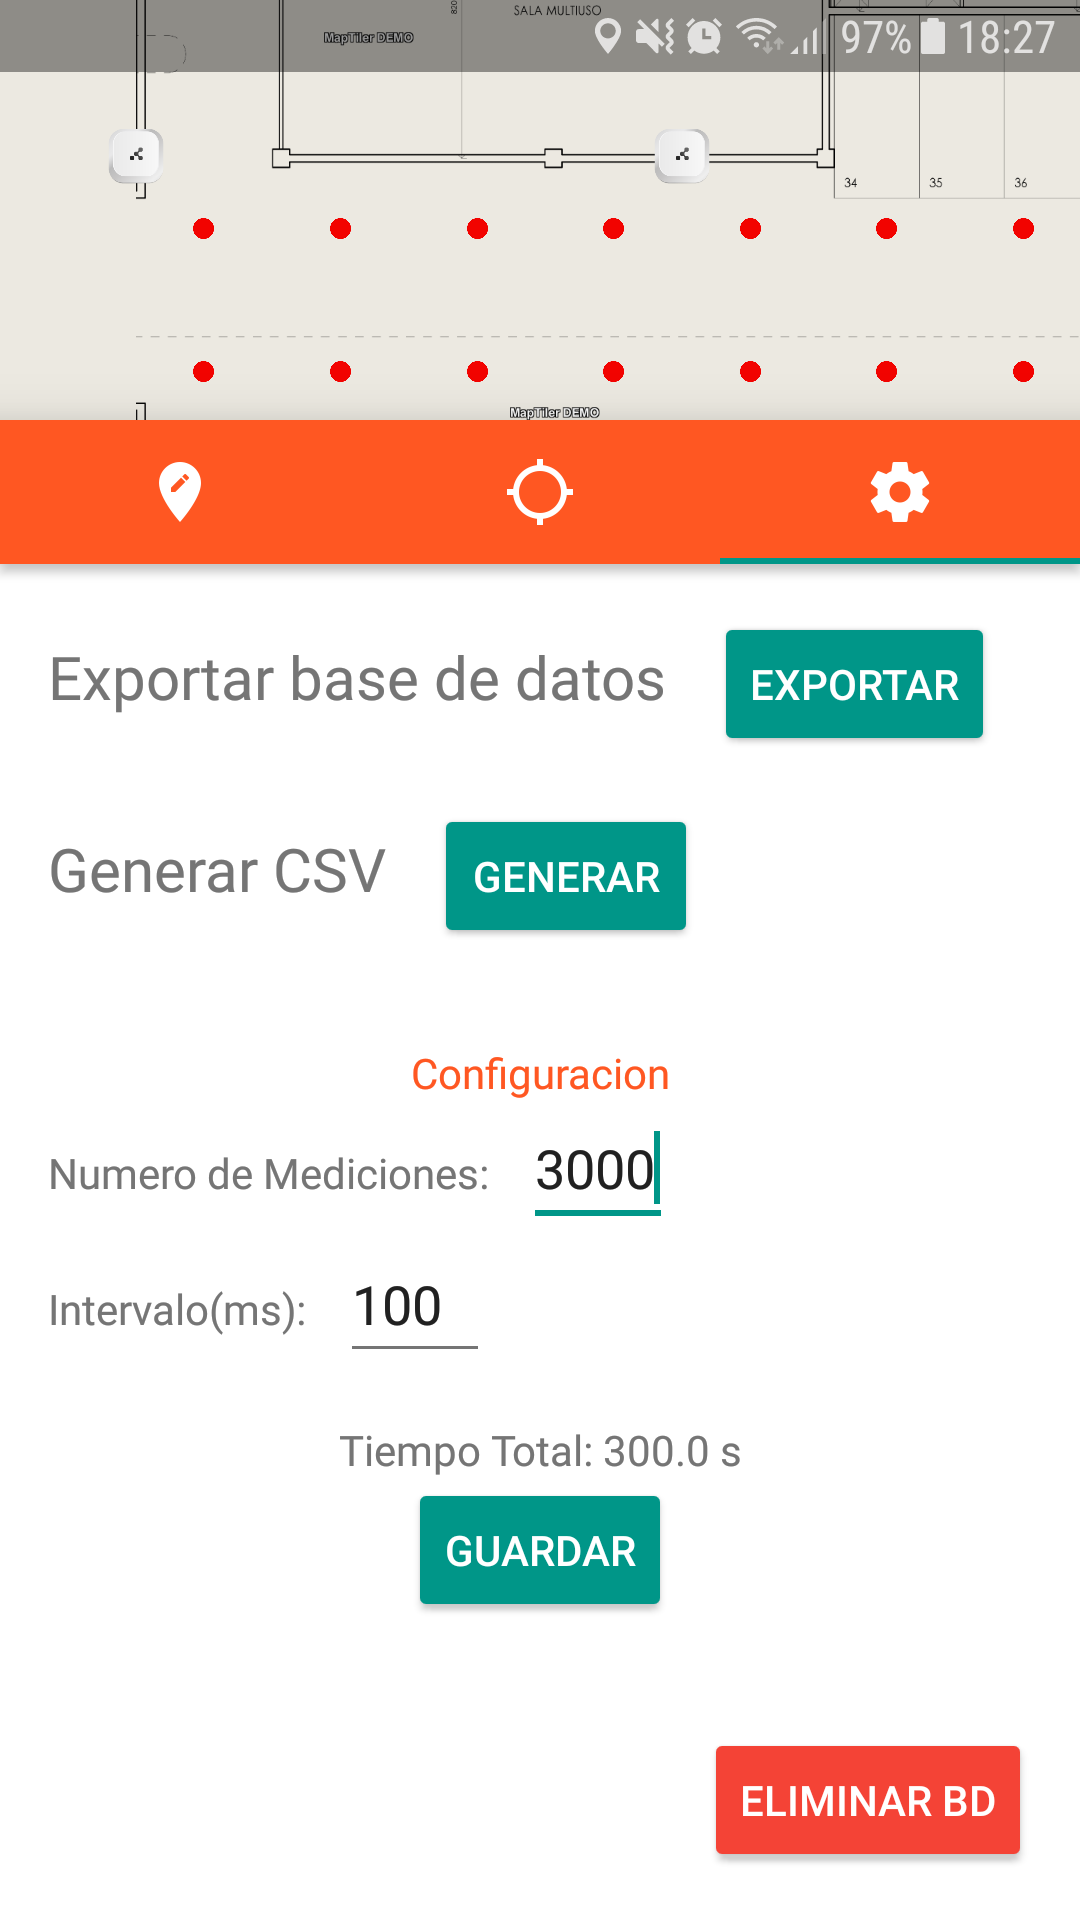
\includegraphics[width=.3\textwidth]{figures/configApp.png}
\caption[abs]{Pestaña de configuración de la aplicación Android, donde se puede configurar el tiempo y exportar la base de datos a CSV\\
{\scriptsize (Fuente: Elaboración Propia)}}
\label{fig:configApp}
\end{figure}


Un ejemplo del archivo CSV obtenido se presenta en la \autoref{fig:ejemploCSV}


\begin{figure}[ht!]
\centering
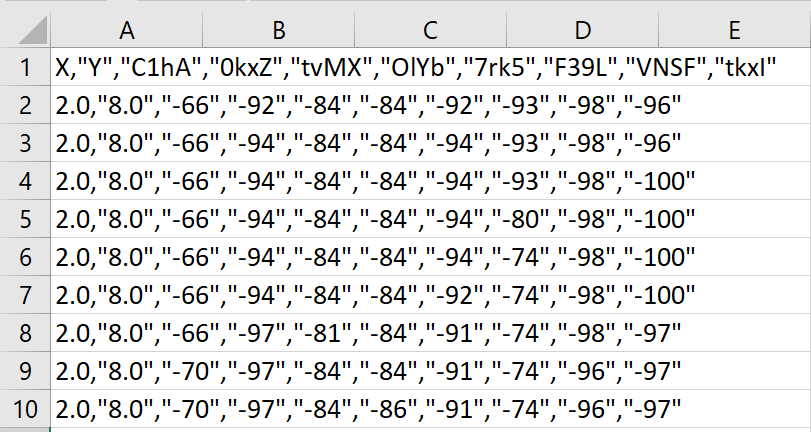
\includegraphics[width=.6\textwidth]{figures/ejemplo_csv.png}
\caption[abs]{Segmento del archivo CSV obtenido a partir de la base de datos. Los primeros dos registros corresponden a las coordenadas y los siguientes, los id unicos de cada Beacon utilizado, con su respectivo en dBm en cada fingerprint. \\
{\scriptsize (Fuente: Elaboración Propia)}}
\label{fig:ejemploCSV}
\end{figure}

Todos estos pasos de recolección son necesarios para los posteriores análisis y entrenamiento de los algoritmos de maquinas de aprendizaje. Para entrenar los clasificadores, se considera entonces cada Beacon en un registro como un feature, es decir, un atributo que funcionara como predictoria para la clasificación. Las etiquetas de cada registro puede corresponder tanto a $X$ como a $Y$, entonces debe entrenarse en ambos casos, por lo que cada clasificador debe presentar 4 casos, esto es $X$ e $Y$ con PCA y $X$ e $Y$ solo con normalizacion de los datos.


\section{Visualización de los datos obtenidos}

En maquinas de aprendizaje, siempre es bueno analizar los datos para determinar patrones o el comportamiento general de los datos. Claramente no es posible visualizar todas las características de una vez, ya 	que al ser mas de tres dimensiones, es complejo para la visualización humana. Mientras los datos en dos o tres  dimensiones pueden ser graficados e interpretados, los datasets de altas dimensiones no cuentan con la misma suerte, y ellos representan la mayor parte de los problemas existentes. El fin de determinar la estructura de los datos es reconocer por ejemplo algún comportamiento extraño o ruido, el cual posteriormente puede ser removido en el caso de ser necesario. Para permitir la visualización de la estructura del dataset, la dimension debe ser reducida de alguna manera, para ser representada en un plano o el espacio cartesiano, algo que es muy intuitivo a la visualización humana.

Para sobrellevar esto, la manera mas simple es tomar una proyección aleatoria de los datos, es decir, seleccionar los features mas representativos según alguna especie de peso o ranking. Esto permite algún grado de visualización de la estructura de los datos, pero se pierde información que muchas veces puede ser relevante. En este tipo de proyecciones, la estructura mas interesante de los datos se pierde debido a la falta de información, por lo que no se representa el problema completo.

Ademas, existen muchos algoritmos tanto supervisados como no supervisados, que son lineales y permiten la reducción de la dimensionalidad, como son \textbf{PCA},  análisis de componentes independientes, analisis de discriminante lineal(\textbf{LDA}), entre otros. En este trabajo PCA es utilizado para reducir la dimensionalidad y evitar la correlación lineal entre los features de los datos. Estos algoritmos definen formas de realizar proyecciones lineales interesantes de los datos. Aunque estos metodos son frecuentemente utilizados, es importante ademas definir otro tipo de algoritmos que ayuden a establecer si entre todas las variables existen estructuras no lineales.

Para conseguir esto, a continuación se utilizan tecnicas de \textbf{Manifold Learning}, las cuales pueden generalizar los frameworks lineales como PCA para ser sensibles a datos altamente no lineales. Un punto importante a destacar es que la mayor cantidad de algoritmos de este tipo son no supervisados, por lo que pueden encontrar las clases automaticamente y separarlas a partir de los mismos datos, sin necesidad de suministrar las etiquetas de cada fingerprint.

Los algoritmos a comparar no seran abordados en detalle porque no es el objetivo de este trabajo, solo se analizaran sus resultados respectivos. Los algoritmos utilizados son Locally Linear Embedding de tipo standar, ltsa, hessian y modificado. Ademas se utilizan otros cuatro métodos correspondientes a Isomap, \textit{Multi-dimensional Scaling}, \textit{Spectral Embedding} y finalmente \textit{t-distributed Stochastic Neighbor Embedding}(\textbf{t-SNE}). Para utilizar estos métodos en primer lugar se normalizan los datos mediante SKlearn, dejándolos con media igual a cero y varianza unitaria, es decir, datos normalmente distribuidos como se define a continuación:

$$ x^{'} = \frac{x- \overline{x}}{\sigma}$$

Una vez estandarizados los datos, se procede a evaluar los algoritmos en ellos. Cabe destacar que para realizar la evaluación se utilizan las clases de la etiqueta $X$, a pesar de que puede usarse $Y$ igualmente, por lo mismo el numero de clases corresponde a 11. La \autoref{fig:manifold} resume los resultados obtenidos debido a aplicar los algoritmos anteriormente mencionados para una proyeccion en dos componentes, es decir en 2-D, con 10 vecinos, donde los vecinos representan un area o vecindario similar al que utiliza K-NN.

\begin{figure}[ht!]
\centering
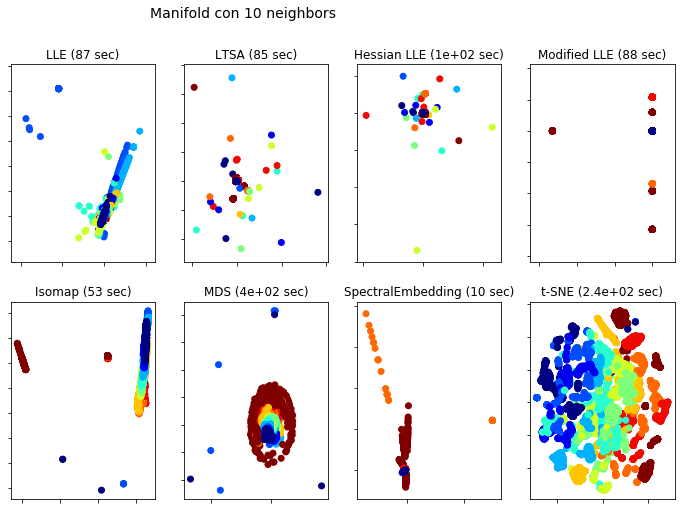
\includegraphics[width=.6\textwidth]{figures/manifold.png}
\caption[abs]{Comparación de los diferentes algoritmos manifold para la reducción de la dimensionalidad con sus respectivos tiempos de ejecución. \\
{\scriptsize (Fuente: Elaboración Propia)}}
\label{fig:manifold}
\end{figure}


Como se aprecia en la figura, la mayor parte de los algoritmos no logran determinar correctamente la estructura de los datos ni mucho menos separar las clases. Los mejores resultados obtenidos en este caso corresponden a Isomap, MDS y t-SNE. Isomap es una extension de MDS y Kernel PCA, y su objetivo es mantener las distancias geodesicas entre todos los puntos. Por su parte MDS busca una representación en la cual las distancias son respetadas segun el espacio original. Finalmente t-SNE convierte la afinidad de los puntos en probabilidades, lo cual lo convierte en uno de los algoritmos mas utilizados, ya que es muy sensible a las estructuras locales en los datos, ademas reduce la tendencia de los datos a agruparse, revelando su estructura de multiples escalas en un solo mapa. Estos Manifolds muestran que los datos presentan una estructura no lineal, debido a los resultados obtenidos principalmente por Isomap y MDS, ya que ellos mantienen  las distancias entre los puntos, por lo que si se lleva al espacio 8-dimensional, MDS muestra una clara separación entre clases anidadas, lo cual en un espacio de mayor dimension, se puede traducir en clases ubicadas cada una en la superficie de un hiperboloide o un hiperplano, lo cual muestra la no linealidad entre los features, sin embargo igualmente se muestran tendencias lineales, pero esto se debe entender como una correlacion lineal local. t-SNE no logra separar las clases de manera correcta, lo cual se puede interpretar como que los datos no son completamente no lineales, y muestran rasgos de linealidad, por lo que PCA se puede utilizar teniendo en cuenta esta aproximación, ya que la correlacion no lineal entre las variables no es fuerte. Con lo anterior, es claro que los valores RSSI ciertamente fluctúan mucho, debido a la gran cantidad de outliers, lo cual es un problema en términos de algoritmos de maquinas de aprendizaje, por situaciones que serán evaluadas posteriormente.


\section{Analisis PCA y LDA}

A pesar de que LDA ya fue descartado previamente debido a que no provee lo que se busca en este trabajo, mas precisamente, disminuir o eliminar la correlación entre puntos adyacentes en la grilla, igualmente se analiza su comportamiento en el dataset obtenido para tener una mejor comprensión de que tanta linealidad presentan los datos, ya que este es un metodo muy efectivo cuando los datos son etiquetados como en este caso. 

Es necesario escalar los datos nuevamente, ya que PCA puede ser susceptible a la escala de los datos y provocar resultados arbitrarios, por lo que se centran los datos,  con media en cero y  varianza unitaria. La resta de la media es necesaria para asegurar que la primera componente principal describe la direccion de maxima varianza, por lo que una media cero es necesaria para asegurar una base en el nuevo subespacio que minimice el error cuadrático medio. Luego de estandarizar los datos, se procede a aplicar PCA y LDA en ellos, de donde se obtiene la \autoref{fig:pca_lda}.

\begin{figure}[ht!]
\centering
\begin{subfigure}{.5\textwidth}
  \centering
  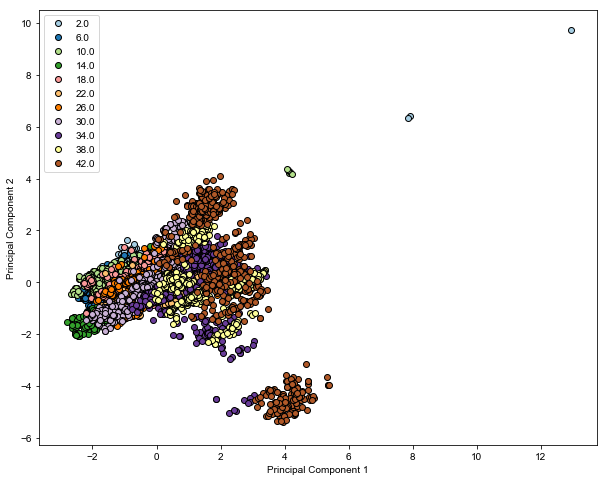
\includegraphics[width=.4\linewidth]{figures/pca.png}
  \caption{PCA}
  \label{fig:sub1}
\end{subfigure}%
\begin{subfigure}{.5\textwidth}
  \centering
  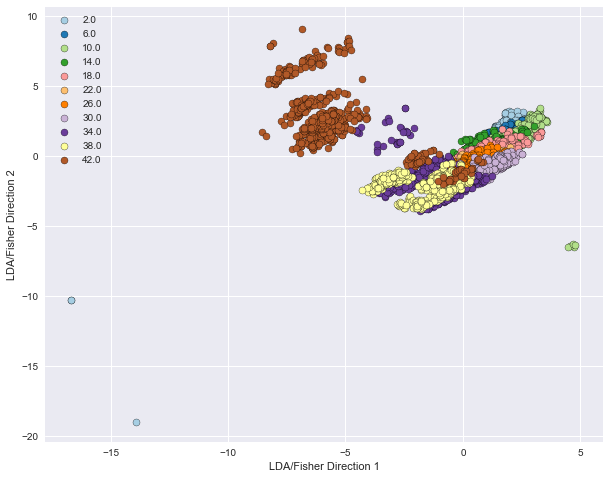
\includegraphics[width=.4\linewidth]{figures/lda.png}
  \caption{LDA}
  \label{fig:sub2}
\end{subfigure}
\caption[abs]{Comparativa entre los algoritmos PCA y LDA aplicado a los datos \\
{\scriptsize (Fuente: Elaboración Propia)}}
\label{fig:pca_lda}
\end{figure}

Como se aprecia en la figura, para PCA se proyecta en las primeras dos componentes principales, lo cual no obtiene buenos resultados, esto puede deberse a muchos factores presentes en los datos, ya que como se menciono anteriormente, los datos no son completamente lineales en el espacio multidimensional, por lo que PCA puede presentar problemas. Ademas, la correlación de los datos es lineal pero solo locamente, en la imagen global, la correlación debe ser de un orden superior(no lineal), por lo que PCA no puede obtener buenos resultados. Tambien es necesario destacar que PCA no esta optimizado para separacion de las clases, y no es precisamente lo que se busca al utilizarlo, la idea principal es reducir la dimensionalidad y evitar la correlacion espacial presente. 

Con respecto a LDA, este si presente buenos resultados, logrando separación entre las clases en gran parte. Esto se debe a que el objetivo de LDA es encontrar una combinación lineal de los features que separe las clases. Ademas, funciona como un clasificador, esto explica los mejores resultados en comparación con PCA. Con lo anterior, es claro la tendencia lineal de los datos, por lo que al aplicar PCA los algoritmos de clasificación deberían presentar resultados positivos debido a que solo se omite información no relevante.

\section{Entrenamiento de clasificadores}

Para el entrenamiento de los clasificadores, se debe tener en cuenta como se menciona anteriormente, que para la gran mayoría de los algoritmos es necesario una normalizacion previa. Esto es particularmente importante en problemas en donde cada atributo puede diferir mucho en orden de magnitud con otras variables. En este caso, no es ciertamente un requisito, ya que los atributos poseen valores de la misma magnitud, porque todas reflejan valores en dBm en un mismo rango, sin embargo igualmente es una buena practica para algoritmos basados en distancia como KNN o SVM, sobre todo por la inclusión del valor 100dbm incorporado para denotar la ausencia de un dispositivo Beacon.

Los clasificadores seleccionados en para este trabajo son Naive Bayes, SVM con Kernel de tipo Radial Basis Function(\textbf{RBF}), SVM con Kernel lineal, K-NN, Arboles de decision, Random Forest, Adaboost, Neural network y QDA. Los parámetros de cada algoritmo son configurados según una búsqueda en grilla, por lo que es necesario correr cada algoritmo múltiples veces en busca de los mejores parametros. Para realizar las pruebas, la forma clásica de realizar machine learning indica tener un training set y un test set, sin embargo en este caso no existe test set, por lo que una opción muy utilizada es separar el conjunto completo de ejemplos en entrenamiento y pruebas, seleccionando un porcentaje del total como test set. Esto funciona muy bien cuando el numero de ejemplos es suficientemente grande, lo cual no ocurre en este caso, por lo que si se quitan datos al training set, es posible que los clasificadores obtengan resultados muy por debajo de como lo harían con la totalidad de los datos.

Para resolver el problema anteriormente descrito, existe una tecnica denominada cross-validation, la cual es muy utilizada y conocida en los campos de inteligencia artificial. El problema principal es que los parametros de cada modelo se ajustan a los datos de entrenamiento lo mejor que pueden, pero al tomar una muestra independiente como datos de prueba desde el mismo training set, generalmente el modelo no se ajusta igual de bien a estos datos de prueba que a los datos de entrenamiento, lo cual se conoce como sobreajuste u \textit{overfitting} y ocurre habitualmente en training set pequeños o cuando el numero de parámetros del modelo es muy grande. Entonces la técnica de cross-validation ayuda a prevenir estas situaciones, ya que a partir de un numero determinado de iteraciones, en cada una de ellas selecciona un conjunto de pruebas de tamaño determinado desde el conjunto total, y al final de todas las iteraciones realiza un promedio de los errores, con lo cual se puede estimar el mejor test score.

En este caso, se decide utilizar cross-validation modificado, el cual utiliza $20\%$ de los datos totales como test set, es decir, lo que habitualmente se conoce como 5-fold cross-validation ya que son 5 iteraciones generales en donde el conjunto de entrenamiento se divide en 5 subconjuntos. La modificación es que en cada iteracion general, ademas se realizan 100 iteraciones adicionales repitiendo el test set, por lo que en total se realiza un total de 500 iteraciones. Esto se debe a que de esta forma se obtienen curvas mas suaves respecto a la media del test y train set. Para obtener el mejor valor en cada caso, se promedian las 100 iteraciones de la primera iteracion global y se obtiene un valor, esto se realiza para cada una de las 5 iteraciones y finalmente se promedian los 5 valores(uno por cada iteracion global) para obtener el mejor valor del train y test set.

Un punto a considerar, es como se menciono anteriormente, las redes neuronales no siguen este procedimiento debido que sklearn no posee este tipo de técnicas, por lo que se usa Tensorflow. Tensorflow tiene sus propios método de validación y los parámetros en este caso son configurados mediante ensayo y error, debido a que esta forma presenta buenos resultados en redes neuronales profundas debido a su complejidad.

Los gráficos obtenidos se muestran conjuntamenteen la \autoref{fig:comparativa_clasificadores}.

\begin{figure}[ht!]
\centering
\begin{subfigure}{.5\textwidth}
  \centering
  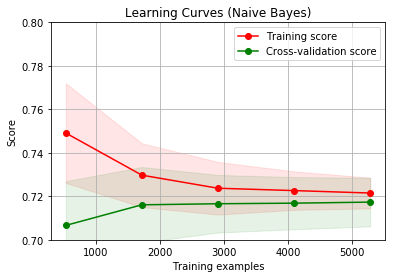
\includegraphics[width=.8\linewidth]{figures/NB.png}
  \caption{Naive Bayes}
  \label{fig:sub1}
\end{subfigure}%
\begin{subfigure}{.5\textwidth}
  \centering
  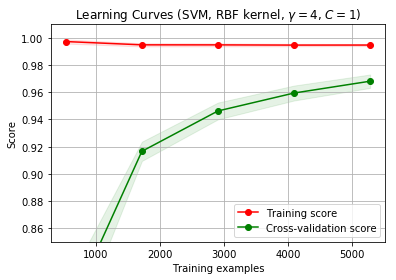
\includegraphics[width=.8\linewidth]{figures/SVM-RBF.png}
  \caption{SVM RBF}
  \label{fig:sub2}
\end{subfigure}

\begin{subfigure}{.5\textwidth}
  \centering
  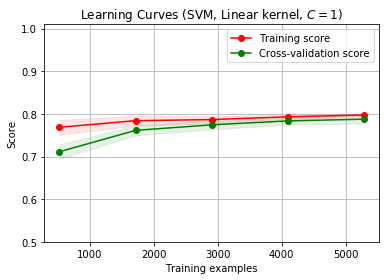
\includegraphics[width=.8\linewidth]{figures/SVM-Lineal.png}
  \caption{SVM Lineal}
  \label{fig:sub1}
\end{subfigure}%
\begin{subfigure}{.5\textwidth}
  \centering
  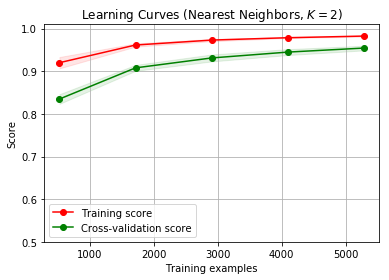
\includegraphics[width=.8\linewidth]{figures/knn-results.png}
  \caption{K-NN}
  \label{fig:sub2}
\end{subfigure}

\begin{subfigure}{.5\textwidth}
  \centering
  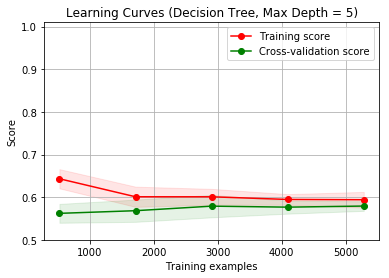
\includegraphics[width=.8\linewidth]{figures/decision-tree.png}
  \caption{Decision Tree}
  \label{fig:sub1}
\end{subfigure}%
\begin{subfigure}{.5\textwidth}
  \centering
  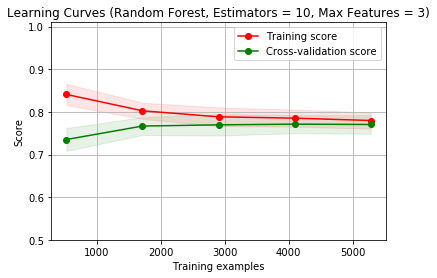
\includegraphics[width=.8\linewidth]{figures/random-forest.png}
  \caption{Random Forest}
  \label{fig:sub2}
\end{subfigure}

\begin{subfigure}{.5\textwidth}
  \centering
  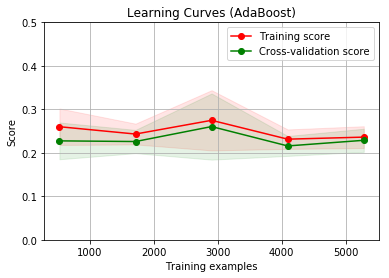
\includegraphics[width=.8\linewidth]{figures/adaboost.png}
  \caption{Adaboost}
  \label{fig:sub1}
\end{subfigure}%
\begin{subfigure}{.5\textwidth}
  \centering
  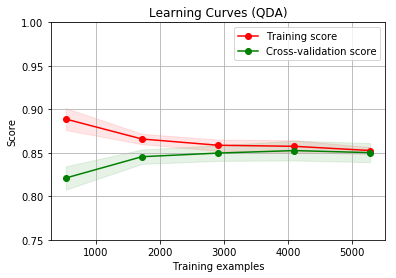
\includegraphics[width=.8\linewidth]{figures/qda.png}
  \caption{QDA}
  \label{fig:sub2}
\end{subfigure}
\caption[abs]{Curvas de aprendizajes obtenidas por cada clasificador \\
{\scriptsize (Fuente: Elaboración Propia)}}
\label{fig:comparativa_clasificadores}
\end{figure}

Se debe señalar que los graficos son para la clasificación sobre la coordenada $X$, sin embargo para $Y$ los resultados son similares, producto de que los datos son esencialmente los mismos, lo único que cambia en el entrenamiento son las clases, así que en términos generales los resultados no deben variar mucho para los algoritmos que realicen una buena clasificación.

Lo que muestran las curvas son los valores medios obtenidos en cada una de las divisiones o \textit{folds}, a partir de las 100 iteraciones. La parte sombreada de cada curva representa la desviacion estandar, es decir, que tanto varian los resultados obtenidos respecto a la media, lo cual sirve para determinar si las pruebas son precisasy no solo depende de la partición realizada en el train set y test set. Por otra parte, para obtener el valor del accuracy se utiliza los \textit{scoring} definidos por defecto en cada clasificador, que en su mayoria corresponde a la similaridad de Jaccard o indice de Jaccard, el compara la similaridad de dos conjuntos y esta definida como el tamaño de la interseccion de los conjuntos dividida por el tamaño de la unión.

$$ J(A, B) = \frac{| \, A \cap B \, |}{| \, A \cup B \,|} =  \frac{| \, A \cap B \, |}{|\, A \,| + |\, B \,|  - | \, A \cap B \, |}$$ 

Se debe notar que el gráfico de entrenamiento y validación de las redes neuronales profundas no se encuentra presente en la \autoref{fig:comparativa_clasificadores}, esto es debido a como se menciona anteriormente, los clasificadores convencionales son implementados en la librería SKlearn, mientras que la red neuronal debe ser procesada en un framework desarrollado exclusivamente para este tipo de redes, por su complejidad computacional y obtener resultados optimizados. Para ello se utiliza Tensorflow y la red utilizada es una red neuronal profunda con dos capas ocultas, la primera de ellas tiene 256 neuronas o nodos, mientras que la segunda capa posee 64 neuronas. Ademas, cabe mencionar que para realizar el entrenamiento de redes neuronales habitualmente no se utiliza cross-validation, ya que cada iteracion supone mucho tiempo, por lo que el entrenamiento total tiene un alto costo computacional, y para grandes bases de datos se utilizan conjuntamente procesadores y tarjetas gráficas para un mejor rendimiento. Por lo anterior, y en vista que cross-validation exige entrenar el modelo múltiples veces, se descarta esta opción por el alto tiempo demandado y se utiliza una separación aleatoria simple en test set y train set, utilizando igual que en los casos anteriores, $20\%$ de los datos como test set.

Los demás parámetros utilizados para entrenar la red neuronal son un numero máximo de pasos o \textit{max-steps} de 20000, que corresponde a los \textbf{epoch}, es decir, las veces que la red se recorre hacia adelante y posteriormente se aplica el algoritmo de backpropagation, mientras aprende los parámetros del modelo. Todo ese proceso entonces es lo que se denomina epoch. Ademas, como optimizador de los parámetros, se utiliza gradiente descendente, con un \textit{learning rate}  igual a $\alpha = 0.3$ . Tambien se define un \textit{batch size} igual a 32, esto representa que el algoritmo aprenderá paulatinamente en subconjuntos de datos de tamaño igual a 32. Esto se conoce como mini-batch Gradient Descent y el error se calcula sobre cada batch, al igual que la actualización de parámetros. La principal ventaja es que al suministrar datos paulatinamente, la actualización de parámetros es mucho mas frecuentemente, lo que ayuda en la convergencia y asi no quedar estancado en mínimos locales. Ademas ayuda a no mantener simultáneamente todos los datos en memoria, por lo que es mucho mas eficiente en términos de memoria y procesamiento.

Con respecto a la estructura de la red, esta se configura como una \textit{input layer} de tamaño del numero de atributos, en este caso corresponde a 8, debido a los 8 beacons. Posteriormente, vienen las dos capas ocultas y finalmente la \textit{output layer}, la cual tiene como objetivo principal entregar probabilidades a cada clase, es decir, por cada clase retorna un valor entre 0 a 1, y entre todas las clases suman 1, por lo que según el mayor valor se puede determinar la clase mas probable. Para entrenar la red se utilizan la \textit{loss function} denominada \textbf{cross entropy}, la que es muy utilizada en redes neuronales por que reduce el problema de aprendizaje presentado por la función de costo cuadrática, también muy utilizada en regresión.

La estructura de la red puede visualizarse en la \autoref{fig:nn_estructura}.

\begin{figure}[ht!]
\centering
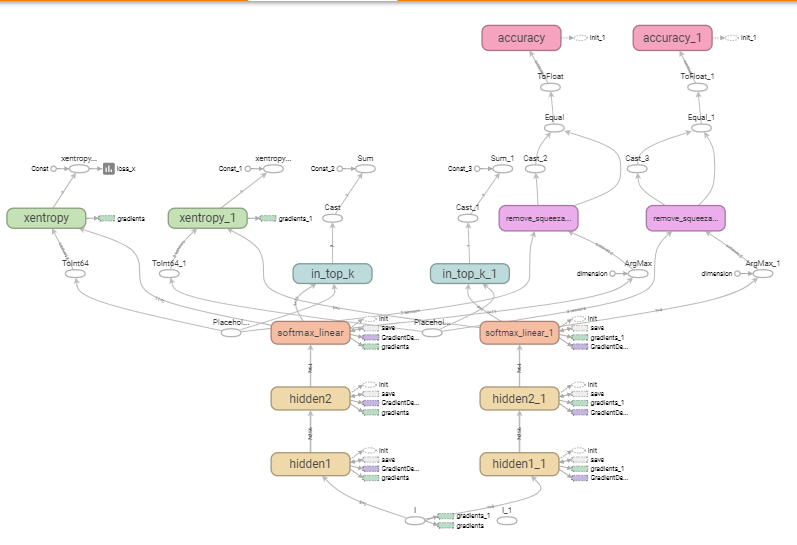
\includegraphics[width=.6\textwidth]{figures/nn_estructura.png}
\caption[abs]{Estructura de las redes neuronales construidas. En la figura se muestran ambas, tanto X como Y \\
{\scriptsize (Fuente: Elaboración Propia)}}
\label{fig:nn_estructura}
\end{figure}

En la imagen se muestra la estructura de la red construida y extraída del visor \textbf{Tensorboard}, un addon de Tensorflow para la visualización de gráficos, grafos, histogramas, entre otros. Se debe notar que existen dos redes paralelas, esto se debe a que las redes neuronales para predecir la clase de X y la clase de Y se entrenan simultáneamente, por esto aparecen juntas en la imagen, pero cada una tiene su propio entrenamiento y evaluación.

Con todos estos puntos definidos, se muestra los resultados obtenidos en el entrenamiento de la red neuronal profunda. La \autoref{nn_metrics} exhibe esta situación.


\begin{figure}[ht!]
\centering
\begin{subfigure}{.5\textwidth}
  \centering
  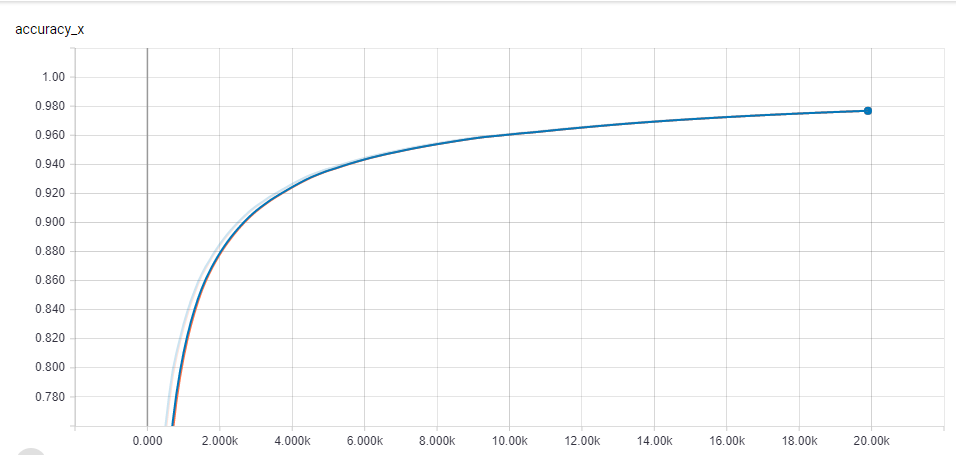
\includegraphics[width=.8\linewidth]{figures/nn_plot.png}
  \caption{Accuracy}
  \label{fig:sub1}
\end{subfigure}%
\begin{subfigure}{.5\textwidth}
  \centering
  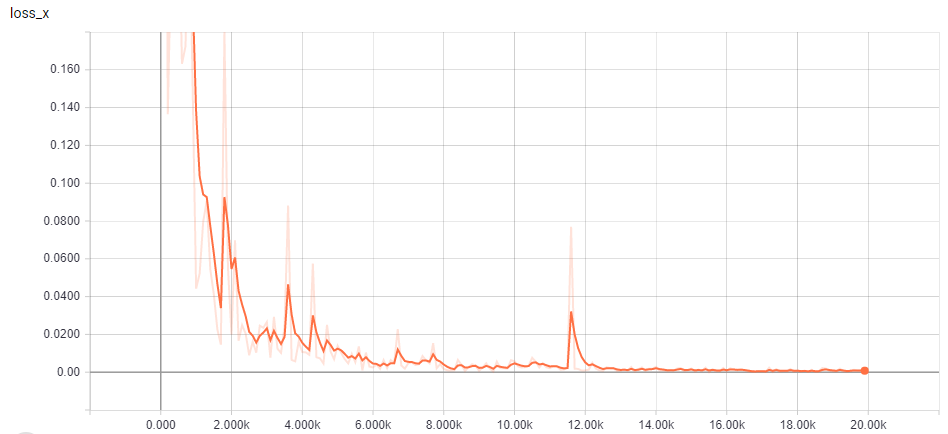
\includegraphics[width=.8\linewidth]{figures/nn_loss.png}
  \caption{Loss}
  \label{fig:sub2}
\end{subfigure}
\caption[abs]{Accuracy y Loss(Costo) obtenidos en el entrenamiento de la red neuronal profunda con dos capas ocultas. \\
{\scriptsize (Fuente: Elaboración Propia)}}
\label{fig:nn_metrics}
\end{figure}

Debe tenerse en cuenta que para la accuracy, los resultados de entrenamiento y pruebas están en la imagen simultaneamente, pero los resultados son tan similares que se sobrepone uno por encima de otro, sin embargo la accuracy sobre el train set es siempre superior(aunque por muy poco) a la accuracy del test set. La funcion de costo o \textit{Loss function} muestra como la red va aprendiendo a medida de los epoch, ya que lo que se busca es minimizar este valor, el cual expresa el costo del modelo o que tan distante es este a los resultados esperados. Como se menciona anteriormente, esta función de costo corresponde a cross-entropy.

Con toda la informacion presentada, es claro que los mejores resultados se presentan principalmente en 3 algoritmos, estos son KNN, SVM con kernel RBF y Redes Neuronales profundas. Lo anterior demuestra que los datos efectivamente tienen estructuras no lineales, ya que K-NN no depende especificamente de la estructura de los datos, ya que busca un radio o vecindario de clasificacion. SVM RBF define areas de clasificacion que precisamente son no lineales, por lo que puede buscar mejores representaciones en este tipo de estructuras que los clasificadores lineales. La forma en que modela estas fronteras no lineales es debido a la eleccion del kernel RBF el cual por su funcion de radio basal es flexible en torno a este tipo de regiones. Por ultimo, las redes neuronales pueden aprender de datos no lineales debido a sus funciones de activación que precisamente son no lineales, ademas de poder aprender patrones mas detallados en cada capa, por su capacidad de reducir la complejidad y dimensionalidad de los datos.

Para corroborar los resultados visualizados en los gráficos, se realiza la tabla con los mejores valores de accuracy para cada algoritmo. Aunque esto puede ser suficiente, ademas se incorpora el mejor error obtenido en metros, es decir, el error cuadrático medio para cada coordenada respectivamente, ya que aunque la accuracy determina que tanto acierta el algoritmo, igualmente es necesario establecer el error medio, porque es preferible tener un valor de error mas pequeño, debido a que este representa el error presente al momento de la fase online de ubicación. Este error esta expresado en metros y se separa según coordenadas, ya sea X o Y.

\begin{table}[ht!]
\centering
\caption{My caption}
\label{my-label}
\begin{tabular}{|c|c|c|c|c|}
\hline
Algoritmo                     & Accuracy & Error medio X & Error medio Y & Error Absoluto \\ \hline
NN                            & 97.94\%  & 0.1579        & 0.0735        & 0.1741         \\ \hline
$SVM(RBF, C=1, \gamma = 4)$   & 96.81\%  & 0.2254        & 0.1018        & 0.2473         \\ \hline
$KNN(k = 2)$                  & 95.43\%  & 0.9842        & 0.1575        & 0.9967         \\ \hline
QDA                           & 85.25\%  & 5.1103        & 4.7175        & 6.9548         \\ \hline
$SVM(Lineal, C=1)$            & 78.75\%  & 9.3163        & 6.0387        & 11.1022        \\ \hline
Random Forest                 & 77.33\%  & 11.3430       & 3.1409        & 11.7698        \\ \hline
Naive Bayes                   & 71.73\%  & 12.2303       & 9.4836        & 15.4763        \\ \hline
Decision Tree( max depth = 5) & 57.91\%  & 57.8012       & 5.6412        & 58.0758        \\ \hline
Adaboost                      & 26.03\%  & 150.8848      & 6.5333        & 151.0261       \\ \hline
\end{tabular}
\end{table}


Efectivamente los mejores clasificadores en términos de accuracy también lo son en error medio, ya sea absoluto o por coordenadas. Para el error absoluto se utiliza la formula de distancia punto a punto, que es lo mas natural debido a la naturaleza del problema.

Con lo anterior, se decide utilizar los tres mejores algoritmos, es decir, que presentan buenos resultados ya sea en accuracy o en error de distancia, los cuales son Red neuronal profunda de dos capas escondidas, SVM con kernel RBF y K-NN. A continuación es necesario realizar el análisis de reducción de la dimension y quitar la correlación de las predictorias mediante el uso de PCA.

\section{Entrenamiento utilizando PCA}

Para el uso de PCA, a pesar de que ya se tiene una noción  de que clasificadores funcionan mejor en este tipo de problemas, igualmente se analiza para los otros tipos de clasificadores, ya que de esta manera se puede evaluar el efecto de aplicarlo en estos, ademas sirven como guía para el análisis posterior.

Lo primero a determinar claramente, es el numero de componentes principales que deben ser utilizadas para disminuir los tiempos de procesamiento y el numero de componentes no ortogonales, es decir, reducir la información redundante total. Para ello se debe seleccionar el mínimo numero de componentes principales, ya que mientras mas se añaden, es mucho mas probable que los datos presenten información no relevante, es decir, ruido e información duplicada. Obviamente, es esencial reducir este tipo de datos para asi mejorar el desempeño de los algoritmos de clasificación.

Para la seleccion, es necesario realizar pruebas que ayuden a la toma de decisiones sobre el numero de componentes principales a utilizar, ya que hasta el momento no existe un algoritmo que lo determine automáticamente, por lo que depende netamente del experimentador y los resultados deseados en términos de accuracy y ahorro de procesamiento. Para ello se proponen tres métodos explicados a continuación. El primer método se basa en la información contextual presente en cada componente principal a través de los valores propios de la matriz de covarianzas. Estos valores propios representan que tanto se explica la varianza en una determinada dirección, en donde la dirección es la determinada por el vector propio asociado al valor propio de esa componente principal. Por lo anterior, a medida que los valores propios de una determinada componente principal incrementan su valor, esta componente principal tiende a tener mas información valiosa en términos generales para el conjunto total de datos. 

Después de aplicar el algoritmo PCA, el espacio de características se mantiene constante según el numero de componentes originales, por lo que si el radiomap se proyecta directamente no hay mejoría y la complejidad computacional incluso puede aumentar. Para la selección, se incorpora una variable $U$, donde esta representa el numero de componentes principales seleccionadas. Como se explica anteriormente, el primer metodo es determinar los valores propios que aportan mas información(varianza), mientras mas alto su valor, la componente principal asociada mantiene mas información valiosa para los datos, es decir, puede interpretarse como la importancia de esa componente. Para determinar los valores propios mas relevantes, estos se determinan segun un criterio muy conocido, el cual es seleccionar aquellos valores propios con valor cercano o mayor a 1. Para ello, se grafican los valores propios en orden descendente:

\begin{figure}[ht!]
\centering
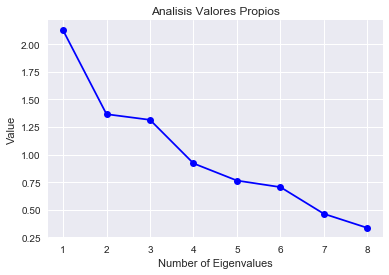
\includegraphics[width=.6\textwidth]{figures/eigenvalues.png}
\caption[abs]{Análisis de los valores propios obtenidos a partir de la matriz de covarianza utilizada en el algoritmo PCA  \\
{\scriptsize (Fuente: Elaboración Propia)}}
\label{fig:manifold}
\end{figure}

Como se observa, los primeros 4 valores propios cumplen la heuristica de selección necesaria, por lo que mantienen la mayor parte de la información del \textit{dataset}.

Para el segundo método, es necesario establecer la suma acumulada porcentual de la varianza explicada, lo cual es sinónimo de el porcentaje de información relevante retenida o acumulada. Para ello, es necesario igualmente utilizar los valores propios que representan la varianza para la selección. La formula a utilizar entonces es:

$$ \frac{\sum_{i=1}^{U}\lambda_{i}}{\sum_{i=1}^{M}\lambda_{i}}  > \xi $$

De donde $\{ \lambda_{1}, \lambda_{2}, ..., \lambda_{M}\}$ corresponden a los valores propios y :

$$\frac{\sum_{i=1}^{U}\lambda_{i}}{\sum_{i=1}^{M}\lambda_{i}}$$

Representa la suma acumulada que retiene la información. Ademas, el limite requerido es $\xi$. Este limite representa la cantidad de información mínima con las cual se acepta el criterio, y habitualmente se elige un valor entre 70 a 80\%. Para esto se muestra la  \autoref{fig:varianza_ratio} la cual describe esta situación.

\begin{figure}[ht!]
\centering
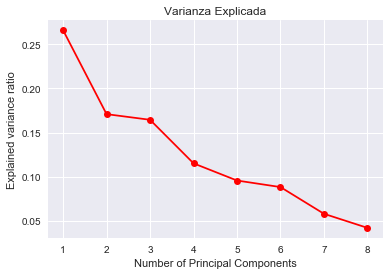
\includegraphics[width=.6\textwidth]{figures/varianza_ratio.png}
\caption[abs]{Proporcion de la varianza explicada respecto a la varianza total para cada componente ordenada por su valor en orden descendente  \\
{\scriptsize (Fuente: Elaboración Propia)}}
\label{fig:varianza_ratio}
\end{figure}

Como se aprecia en la imagen anterior, las primeras 5 componentes principales retienen la cantidad de información especificada según el limite impuesto $\xi =0.8$. Para clarificar este punto se construye una tabla resumen con los valores propios, la proporción de varianza explicada y la suma acumulada de estas proporciones.

\begin{table}[]
\centering
\caption{My caption}
\label{my-label}
\begin{tabular}{|c|c|c|c|c|c|c|c|c|}
\hline
Indicador                     & PC1    & PC2    & PC3    & PC4     & PC5    & PC6    & PC7    & PC8    \\ \hline
Valor Propio                  & 2.1271 & 1.3665 & 1.3154 & 0.92088 & 0.7652 & 0.7058 & 0.4637 & 0.3363 \\ \hline
Proporcion Varianza Explicada & 0.2658 & 0.1707 & 0.1644 & 0.1150  & 0.0956 & 0.0882 & 0.0579 & 0.0420 \\ \hline
Suma Acumulada Proporcion     & 0.2658 & 0.4366 & 0.6010 & 0.7161  & 0.8117 & 0.9000 & 0.9579 & 1.000  \\ \hline
\end{tabular}
\end{table}

Con respecto al tercer método, este se basa en seleccionar las primeras componentes principales según los resultados obtenidos en los clasificadores, por lo que se necesita PCA ya aplicado, no solo basta con la matriz de correlación, si no que los algoritmos completos. Para realizar este método entonces se decide aplicar PCA en todos los algoritmos de clasificación nombrados anteriormente, con ellos se pretende establecer los mejores valores de accuracy y en que puntos a nivel de componentes principales, la mayoría de los clasificadores establecen sus mejores puntuaciones en términos de accuracy, por lo que añadir mas componentes no provoca una mejoría significativa.

La \autoref{fig:comparativa_pca} muestra la comparativa de los clasificadores.

\begin{figure}[ht!]
\centering
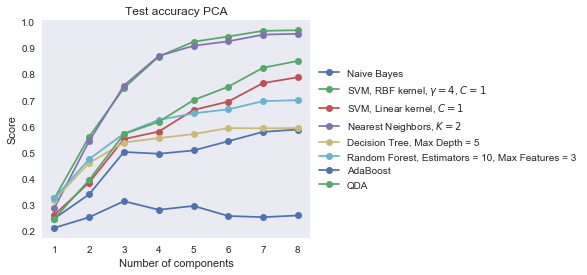
\includegraphics[width=.6\textwidth]{figures/comparativa_clasificadores_pca.png}
\caption[abs]{Comparativa de resultados obtenidos por los clasificadores utilizando PCA  \\
{\scriptsize (Fuente: Elaboración Propia)}}
\label{fig:comparativa_pca}
\end{figure}

Según la comparativa, es claro que la mayoría de los clasificadores presentan una gran mejoría hasta la quinta componente, y posteriormente la ganancia no es significante respecto a la información aportada a los respectivos algoritmos. Esto indica al igual que los otros métodos de selección, que a partir de la quinta componente la varianza aportada no es realmente significativa, por lo que puede reducirse la dimensionalidad de los datos a 5, ya que los tres métodos utilizados presentan resultados similares y coinciden en este valor de componentes principales.

Posteriormente, se procede a evaluar según el procedimiento realizado anteriormente para los clasificadores sin utilizar PCA. Los resultados obtenidos en cada clasificador se muestran en la \autoref{fig:comparativa_clasificadores_pca}. Se debe destacar que los hiperparametros de cada algoritmo no fueron cambiados respecto a sus versiones sin utilizar PCA.


\begin{figure}[ht!]
\centering
\begin{subfigure}{.5\textwidth}
  \centering
  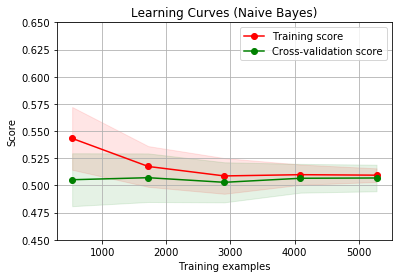
\includegraphics[width=.8\linewidth]{figures/NB_PCA.png}
  \caption{Naive Bayes PCA}
  \label{fig:sub1}
\end{subfigure}%
\begin{subfigure}{.5\textwidth}
  \centering
  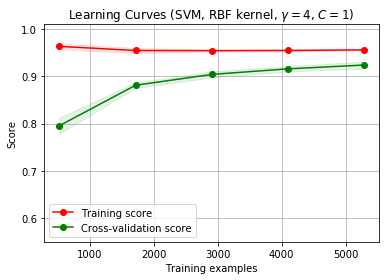
\includegraphics[width=.8\linewidth]{figures/SVM-RBF-PCA.png}
  \caption{SVM RBF PCA}
  \label{fig:sub2}
\end{subfigure}

\begin{subfigure}{.5\textwidth}
  \centering
  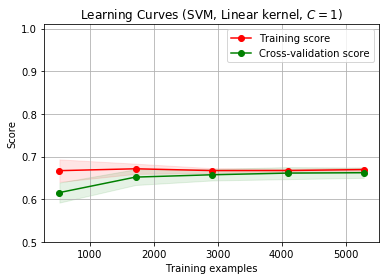
\includegraphics[width=.8\linewidth]{figures/SVM-Lineal-PCA.png}
  \caption{SVM Lineal PCA}
  \label{fig:sub1}
\end{subfigure}%
\begin{subfigure}{.5\textwidth}
  \centering
  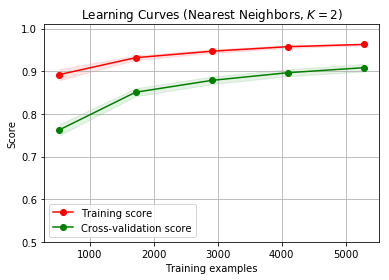
\includegraphics[width=.8\linewidth]{figures/knn-results-PCA.png}
  \caption{K-NN PCA}
  \label{fig:sub2}
\end{subfigure}

\begin{subfigure}{.5\textwidth}
  \centering
  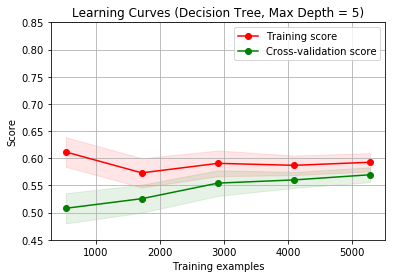
\includegraphics[width=.8\linewidth]{figures/decision-tree-PCA.png}
  \caption{Decision Tree PCA}
  \label{fig:sub1}
\end{subfigure}%
\begin{subfigure}{.5\textwidth}
  \centering
  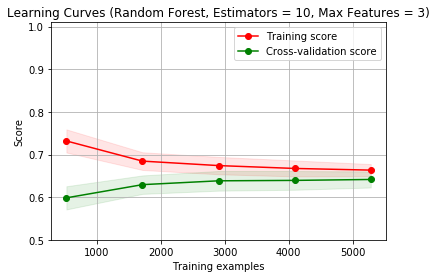
\includegraphics[width=.8\linewidth]{figures/random-forest-PCA.png}
  \caption{Random Forest PCA}
  \label{fig:sub2}
\end{subfigure}

\begin{subfigure}{.5\textwidth}
  \centering
  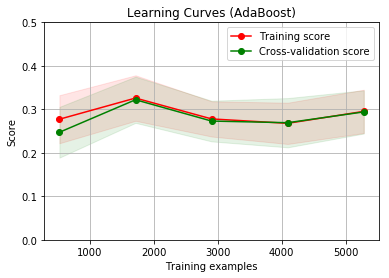
\includegraphics[width=.8\linewidth]{figures/adaboost-PCA.png}
  \caption{Adaboost PCA}
  \label{fig:sub1}
\end{subfigure}%
\begin{subfigure}{.5\textwidth}
  \centering
  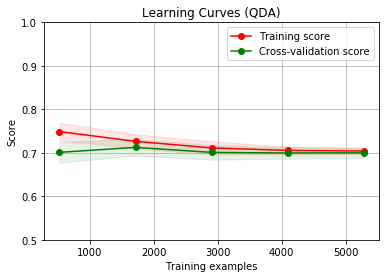
\includegraphics[width=.8\linewidth]{figures/qda-PCA.png}
  \caption{QDA PCA}
  \label{fig:sub2}
\end{subfigure}
\caption[abs]{Curvas de aprendizajes obtenidas por cada clasificador utilizando PCA con 5 componentes\\
{\scriptsize (Fuente: Elaboración Propia)}}
\label{fig:comparativa_clasificadores_pca}
\end{figure}

En este caso, se obtienen resultados similares a los obtenidos sin utilizar PCA, esto es un indicativo de que la eleccion de las componentes principales es correcto. Para analizar las redes neuronales utilizando PCA se procede a graficar la accuracy y la función de perdida al igual que en casos anteriores.

\begin{figure}[ht!]
\centering
\begin{subfigure}{.5\textwidth}
  \centering
  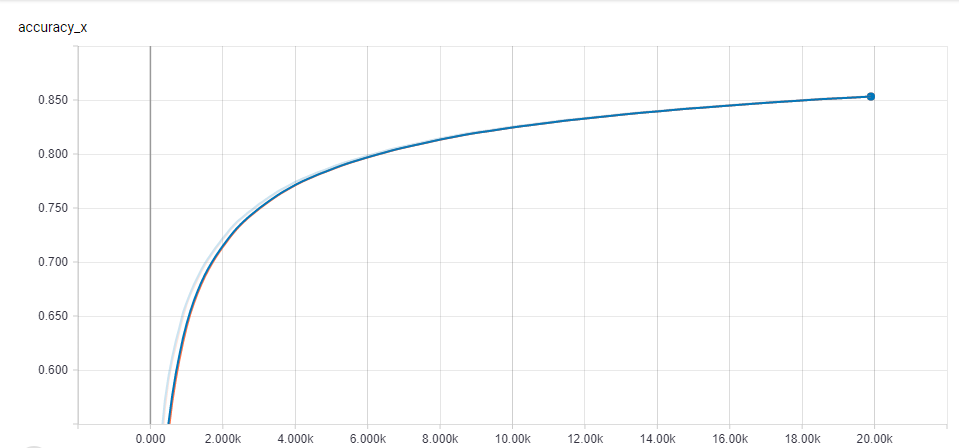
\includegraphics[width=.8\linewidth]{figures/nn_plot_pca.png}
  \caption{Accuracy PCA}
  \label{fig:sub1}
\end{subfigure}%
\begin{subfigure}{.5\textwidth}
  \centering
  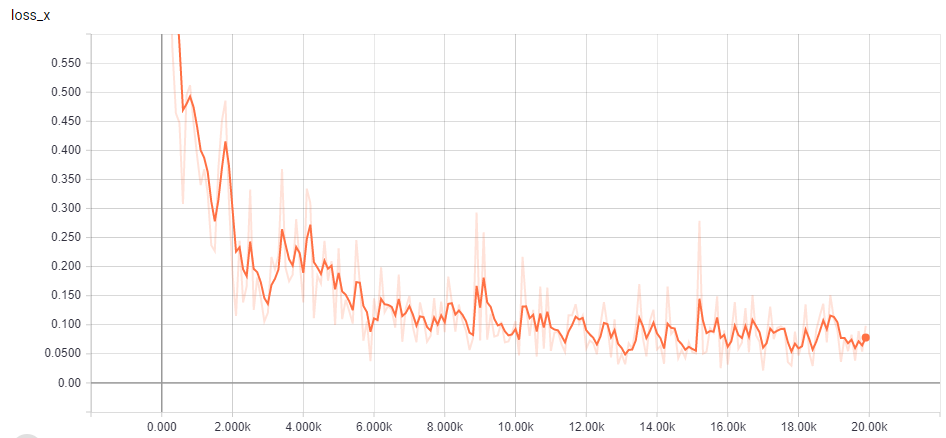
\includegraphics[width=.8\linewidth]{figures/nn_loss_pca.png}
  \caption{Loss PCA}
  \label{fig:sub2}
\end{subfigure}
\caption[abs]{Accuracy y Loss(Costo) obtenidos en el entrenamiento de la red neuronal profunda con dos capas ocultas utilizando PCA con 5 componentes principales. \\
{\scriptsize (Fuente: Elaboración Propia)}}
\label{fig:nn_metrics_pca}
\end{figure}

Al igual que los clasificadores convencionales, los resultados son muy similares a los obtenidos mediante clasificadores sin utilizar PCA. Esto es un indicativo de que la eleccion de las componentes principales es acertado. Para corroborar esto se construye la tabla \autoref{tabla-pca} la cual es simil a la \autoref{my-label}

\begin{table}[ht!]
\centering
\caption{My caption}
\label{tabla-pca}
\begin{tabular}{|c|c|c|c|c|}
\hline
Algoritmo                     & Accuracy & Error medio X & Error medio Y & Error Absoluto \\ \hline
NN                            & 93\%  & 1.8956        & 0.6589        & 2.0068         \\ \hline
$SVM(RBF, C=1, \gamma = 4)$   & 92.39\%  & 2.4581  & 0.7830        & 2.5797         \\ \hline
$KNN(k = 2)$                  & 90.83\%  & 2.1381 & 0.4872        & 2.1929         \\ \hline
QDA                           & 71.25\%  & 15.9418 & 9.3042        & 18.4583         \\ \hline
$SVM(Lineal, C=1)$            & 66.20\%  & 19.5878 & 10.4824        & 22.2162        \\ \hline
Random Forest                 & 64.15\%  & 21.3284 & 5.4472        & 22.0130       \\ \hline
Decision Tree( max depth = 5) & 56.96\%  & 33.5151       & 8.9163       & 34.6808        \\ \hline
Naive Bayes                   & 50.71\%  & 31.3406 & 10.0727        & 32.9194        \\ \hline
Adaboost                      & 32.20\%  & 73.9345 & 9.3042       & 74.5176       \\ \hline
\end{tabular}
\end{table}

Los valores obtenidos entonces demuestran que a pesar de que la accuracy se reduce solo un poco, los valores de error medio decrementan significativamente en el contexto del problema abordado, ya que para el posicionamiento en interiores se espera un error lo mas pequeño posible, ya que esto significa una mejor localizacion. Por lo anterior, se debe tener en cuenta estos factores al momento de seleccionar las componentes principales, ya que al perder informacion, se pierde exactitud en las mediciones, lo que repercute significativamente al momento de realizar pruebas reales. 

El comportamiento en términos generales sigue el mismo patrón que al no aplicar técnicas de reducción de dimensionalidad, es decir, los clasificadores mantienen el orden realtivo en cuanto a accuracy y nuevamente los clasificadores capaces de distinguir patrones no lineales en los datos son los dominantes, lo cual prueba esta características de los datos. También se debe notar que los tres primeros lugares corresponden nuevamente a redes neuronales profundas, maquina de vectores de soporte con kernel RBF y finalmente vecinos mas cercanos con $k=2$. 

Por lo anterior, se decide utilizar los tres clasificadores NN, SVM y KNN para realizar la experimentación en el estacionamiento descrito anteriormente. A continuación se define el método utilizado para realizar las pruebas.


\section{Fase Online}

Para realizar las pruebas dentro del recinto es necesario establecer el marco a utilizar para determinar la exactitud y precision del sistema. En primer lugar se debe tener en cuenta que no hay forma de determinar el error absoluto, producto de que para ello se debe proporcionar la posición real, lo cual es contradictorio, ya que esto es precisamente lo que se busca. Existen métodos de buscar este error, por ejemplo \citep{Ugave} describe una forma de medir los errores mediante el uso de la creación de caminos predefinidos. Luego para medir la precision, se infiere la pocision estimada cada 10 metros siguiendo la trayectoria definida. Luego, con la posicion estimada y la posicion teórica determinada por el camino establecido, se puede obtener la distancia que representa el error, la cual esta definida mediante el vector perpendicular desde la trayectoria definida hasta el punto predicho. 

Otro tipo de enfoque es utilizar el tiempo recorrido y mediante las ecuaciones de movimiento obtener una posición aproximada que puede ser comparada con la inferida por los algoritmos de maquinas de aprendizaje.

El problema con estos enfoques, es que se basan en propiedades del experimentador, como por ejemplo utilizar sensores basados en detección de pasos, lo cual no es del todo preciso, o también al utilizar las ecuaciones de posición se requiere que la velocidad del experimentador sea constante y medir exactamente en un instante indicado, lo cual dificulta mucho las pruebas y también agrega factores de error externos lo que se traduce en resultados ruidosos y poco fidedignos. Entonces lo que se propone para determinar los resultados son dos formas llamadas método estático y método dinámico. En el método estático lo que se hace es permanecer quieto en un determinado punto durante un tiempo predefinido. El tiempo utilizado en este caso corresponde a 15 minutos, y el punto es especifico es $(22, 12)$. Para el caso del método dinámico, lo que se busca es abarcar la mayor cantidad de puntos posibles y establecer de ante mano el punto en el cual se realizaran las mediciones a través de una caminata. En este caso se decide hacer una caminata a través de todos los 44 puntos posibles de izquierda a derecha, arriba a abajo durante un tiempo de 30 minutos.

Para realizar las pruebas se adiciona una pantalla a la aplicacion precisamente para la fase Online, la \autoref{fig:fase_online} muestra esta situación.

\begin{figure}[ht!]
\centering
\begin{subfigure}{.3\textwidth}
  \centering
  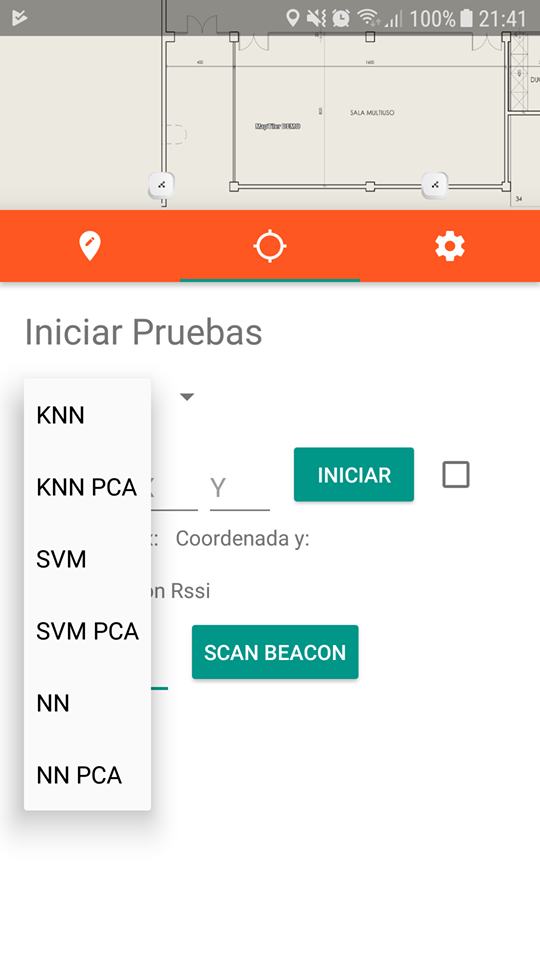
\includegraphics[width=.8\linewidth]{figures/fase_online1.png}
  \caption{Selección algoritmo}
  \label{fig:online1}
\end{subfigure}%
\begin{subfigure}{.3\textwidth}
  \centering
  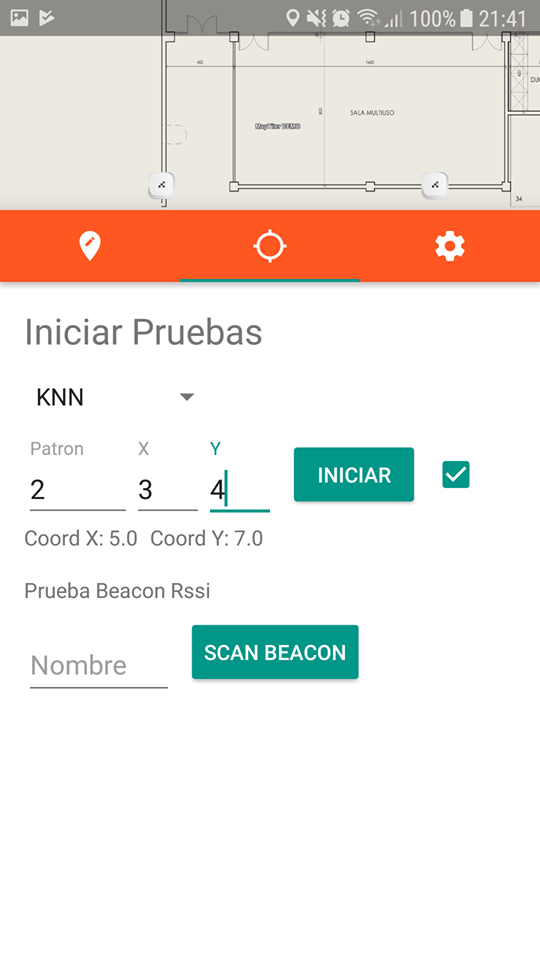
\includegraphics[width=.8\linewidth]{figures/fase_online2.png}
  \caption{Elección patrón}
  \label{fig:online2}
\end{subfigure}
\begin{subfigure}{.3\textwidth}
  \centering
  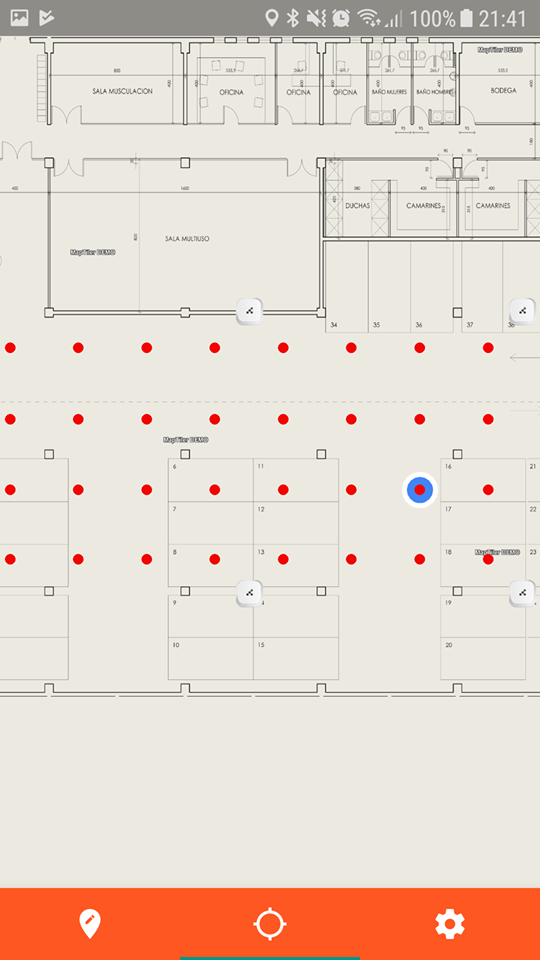
\includegraphics[width=.8\linewidth]{figures/fase_online3.png}
  \caption{Posicionamiento real}
  \label{fig:online3}
\end{subfigure}
\caption[abs]{Pantalla utilizada en la fase Online para la realizacion de las pruebas de experimentos reales \\
{\scriptsize (Fuente: Elaboración Propia)}}
\label{fig:fase_online}
\end{figure}

Como se observa en la imagen \autoref{fig:fase_online}, en primer lugar se debe elegir el algoritmo a utilizar en el posicionamiento, luego seleccionar el patrón para elegir el punto en donde se realizaran las pruebas y finalmente iniciar, lo cual comienza a posicionar al usuario en tiempo real. Para el método dinámico los pasos son igual, solo se debe utilizar el \textit{checkbox} al lado del botón iniciar y cambiar progresivamente el punto a utilizar mientras se sigue el camino de predicción.

A pesar de que se selecciona un algoritmo para la visualizacion del posicionamiento, internamente la aplicación ejecuta todos los algoritmos mostrados, es decir NN, SVM y KNN con sus respectivas versiones utilizando PCA. El fin de esto es ahorrar tiempo, ya que de esta forma se pueden obtener los resultados para todos los algoritmos concurrentemente sin necesidad de ejecutarlos de manera secuencial. Luego la aplicación tiene la capacidad de crear archivos de \textit{log}, es decir, guardar los resultados obtenidos. El formato de estos archivos es diseñado para su posterior análisis. La primera linea contiene el tipo de método, estático o dinámico. La siguiente linea de texto muestra el punto teórico con el cual se comparan los datos. Posteriormente el nombre del algoritmo, luego una lista de valores de la posición $X$, a continuación una lista de valores $Y$ y finalmente el tiempo de ejecución del algoritmo. Para cada algoritmo se repite esta estructura, en el orden mostrado en la \autoref{fig:online1}. Claramente la lista de valores $X$ e $Y$ tienen las mismas dimensiones y forman las predicciones finales según su posición relativa, es decir, el primer elemento de la lista $X_{1}$ con el primer elemento de la lista $Y_{1}$ forman el primer punto predicho por el algoritmo $(X_{1}, Y_{1})$. 

Para clarificar esto, la \autoref{online_results} muestra un extracto de un archivo obtenido luego de realizar la experimentación de la fase online. Este archivo es de tipo dinámico, con lo que contiene múltiples puntos de clasificación.

\begin{figure}[ht!]
\centering
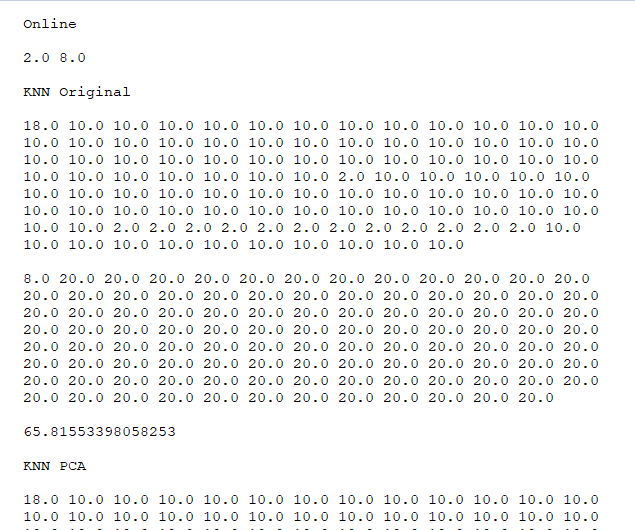
\includegraphics[width=.6\textwidth]{figures/online-results.png}
\caption[abs]{Archivo obtenido en la experimentación online  \\
{\scriptsize (Fuente: Elaboración Propia)}}
\label{fig:online_results}
\end{figure}


